\documentclass[11pt]{article}

\usepackage[final]{acl}
\usepackage{times}
\usepackage{latexsym}
\usepackage[T1]{fontenc}
\usepackage[utf8]{inputenc}
\usepackage{microtype}
\usepackage{inconsolata}
\usepackage{graphicx}
\usepackage{booktabs}
\usepackage{multirow}
\usepackage{amsmath}
\usepackage{amssymb}
\usepackage{xcolor}
\usepackage{enumitem}

\title{AmanaMT: Translation Direction Predicts Automatic Metric Reliability}

\author{Isaac Thompson \\
  Brigham Young University \\
  \texttt{it238@byu.edu}}

\begin{document}
\maketitle
% AUTO-GENERATED by scripts/render_macros.py — DO NOT EDIT BY HAND
% Single source of truth: results/paper_stats.json
% To change a value: fix the analysis script that produced it, rerun the
% full pipeline (see this script's docstring), then rerun render_macros.py.
%
\newcommand{\BaselineValCoreMinPearson}{0.867}  % wmt_baseline_validation_segment_level.csv
\newcommand{\BaselineValCoreMinSpearman}{0.837}  % wmt_baseline_validation_segment_level.csv
\newcommand{\BaselineValMinPearson}{0.572}  % wmt_baseline_validation_segment_level.csv
\newcommand{\BaselineValMinSpearman}{0.623}  % wmt_baseline_validation_segment_level.csv
\newcommand{\BaselineValNChecks}{8}  % wmt_baseline_validation_segment_level.csv
\newcommand{\BeatsCometEntoXAgglutin}{6}  % recompute:table4_wins
\newcommand{\BeatsCometEntoXFusional}{7}  % recompute:table4_wins
\newcommand{\BeatsCometEntoXTotal}{13}  % recompute:table4
\newcommand{\BeatsCometXtoEnAgglutin}{6}  % recompute:table4_wins
\newcommand{\BeatsCometXtoEnFusional}{6}  % recompute:table4_wins
\newcommand{\BeatsCometXtoEnIsolating}{1}  % recompute:table4_wins
\newcommand{\CellCIEntoXAgglutinHi}{1.00}  % direction_separated_cell_cis.csv
\newcommand{\CellCIEntoXAgglutinLo}{1.00}  % direction_separated_cell_cis.csv
\newcommand{\CellCIEntoXFusionalHi}{1.00}  % direction_separated_cell_cis.csv
\newcommand{\CellCIEntoXFusionalLo}{1.00}  % direction_separated_cell_cis.csv
\newcommand{\CellCIXtoEnAgglutinHi}{1.00}  % direction_separated_cell_cis.csv
\newcommand{\CellCIXtoEnAgglutinLo}{1.00}  % direction_separated_cell_cis.csv
\newcommand{\CellCIXtoEnFusionalHi}{1.00}  % direction_separated_cell_cis.csv
\newcommand{\CellCIXtoEnFusionalLo}{0.43}  % direction_separated_cell_cis.csv
\newcommand{\ChrFErrorFreeDE}{0.77}  % surface_similarity.csv
\newcommand{\ChrFErrorFreeHE}{0.77}  % surface_similarity.csv
\newcommand{\CometXcometHeEsMinRho}{0.77}  % recompute:gemba_remap_check
\newcommand{\CsEnDelta}{+0.012}  % simpsons_cs_da.csv
\newcommand{\CsEnPooled}{.288}  % simpsons_cs_da.csv
\newcommand{\CsEnRangeHi}{0.69}  % simpsons_cs_da.csv
\newcommand{\CsEnRangeLo}{-0.01}  % simpsons_cs_da.csv
\newcommand{\DeDelta}{+0.000}  % tier_anomaly.csv
\newcommand{\DeEnCOMETRho}{.383}  % scores_de_en.csv
\newcommand{\DeEnCOMETRhoTbl}{0.383}  % scores_de_en.csv
\newcommand{\DeEnKiwiRho}{.414}  % scores_de_en.csv
\newcommand{\DeEnKiwiRhoTbl}{0.414}  % scores_de_en.csv
\newcommand{\DeEnMetricXRho}{.389}  % scores_de_en.csv
\newcommand{\DeEnN}{134{,}792}  % scores_de_en.csv
\newcommand{\DeRangeHi}{0.50}  % tier_anomaly.csv
\newcommand{\DeRangeLo}{0.32}  % tier_anomaly.csv
\newcommand{\DeWmtTwoOneRho}{.323}  % tier_anomaly.csv
\newcommand{\DeWmtTwoTwoRho}{.456}  % tier_anomaly.csv
\newcommand{\DeWmtTwoZeroRho}{.497}  % tier_anomaly.csv
\newcommand{\DiDValue}{0.036}  % recompute:gaps
\newcommand{\DirMetricBLEUEntoX}{0.303}  % recompute:direction_metric
\newcommand{\DirMetricBLEUPivot}{0.202}  % recompute:direction_metric
\newcommand{\DirMetricBLEUXtoEn}{0.230}  % recompute:direction_metric
\newcommand{\DirMetricCKXXIIIEntoX}{0.650}  % recompute:direction_metric
\newcommand{\DirMetricCKXXIIIPivot}{0.332}  % recompute:direction_metric
\newcommand{\DirMetricCKXXIIIXtoEn}{0.387}  % recompute:direction_metric
\newcommand{\DirMetricCOMETEntoX}{0.605}  % recompute:direction_metric
\newcommand{\DirMetricCOMETPivot}{0.354}  % recompute:direction_metric
\newcommand{\DirMetricCOMETXtoEn}{0.364}  % recompute:direction_metric
\newcommand{\DirMetricChrFEntoX}{0.380}  % recompute:direction_metric
\newcommand{\DirMetricChrFPivot}{0.247}  % recompute:direction_metric
\newcommand{\DirMetricChrFXtoEn}{0.253}  % recompute:direction_metric
\newcommand{\DirMetricMetricXEntoX}{0.671}  % recompute:direction_metric
\newcommand{\DirMetricMetricXPivot}{0.530}  % recompute:direction_metric
\newcommand{\DirMetricMetricXXtoEn}{0.392}  % recompute:direction_metric
\newcommand{\DirMetricxCOMETEntoX}{0.602}  % recompute:direction_metric
\newcommand{\DirMetricxCOMETPivot}{0.340}  % recompute:direction_metric
\newcommand{\DirMetricxCOMETXtoEn}{0.350}  % recompute:direction_metric
\newcommand{\DirMorphCOMETEntoXAgglutin}{0.675}  % recompute:direction_morphology
\newcommand{\DirMorphCOMETEntoXAgglutinCIhi}{0.720}  % recompute:direction_morphology
\newcommand{\DirMorphCOMETEntoXAgglutinCIlo}{0.619}  % recompute:direction_morphology
\newcommand{\DirMorphCOMETEntoXFusional}{0.563}  % recompute:direction_morphology
\newcommand{\DirMorphCOMETEntoXFusionalCIhi}{0.657}  % recompute:direction_morphology
\newcommand{\DirMorphCOMETEntoXFusionalCIlo}{0.446}  % recompute:direction_morphology
\newcommand{\DirMorphCOMETPivotFusional}{0.354}  % recompute:direction_morphology
\newcommand{\DirMorphCOMETPivotFusionalCIhi}{0.466}  % recompute:direction_morphology
\newcommand{\DirMorphCOMETPivotFusionalCIlo}{0.242}  % recompute:direction_morphology
\newcommand{\DirMorphCOMETXtoEnAgglutin}{0.440}  % recompute:direction_morphology
\newcommand{\DirMorphCOMETXtoEnAgglutinCIhi}{0.538}  % recompute:direction_morphology
\newcommand{\DirMorphCOMETXtoEnAgglutinCIlo}{0.313}  % recompute:direction_morphology
\newcommand{\DirMorphCOMETXtoEnFusional}{0.292}  % recompute:direction_morphology
\newcommand{\DirMorphCOMETXtoEnFusionalCIhi}{0.438}  % recompute:direction_morphology
\newcommand{\DirMorphCOMETXtoEnFusionalCIlo}{0.156}  % recompute:direction_morphology
\newcommand{\DirMorphCOMETXtoEnIsolating}{0.462}  % recompute:direction_morphology
\newcommand{\EntoXTotalPairs}{13}  % recompute:table4
\newcommand{\EtaSqDir}{0.309}  % recompute:direction_morphology
\newcommand{\EtaSqInteract}{0.618}  % recompute:direction_morphology
\newcommand{\EtaSqMorph}{0.073}  % recompute:direction_morphology
\newcommand{\GapCometBleuAgglutinEntoX}{0.351}  % recompute:gaps
\newcommand{\GapCometBleuAgglutinXtoEn}{0.151}  % recompute:gaps
\newcommand{\GapCometBleuFusionalXtoEn}{0.119}  % recompute:gaps
\newcommand{\GapDirAgglutin}{0.235}  % recompute:gaps
\newcommand{\GapDirFusional}{0.271}  % recompute:gaps
\newcommand{\GapEsKiwiComet}{-0.142}  % recompute:hebrew
\newcommand{\GapHeKiwiComet}{-0.173}  % recompute:hebrew
\newcommand{\GapKMMetricXBleu}{0.174}  % recompute:table4
\newcommand{\GapZHMetricXBleu}{0.478}  % recompute:table4
\newcommand{\HeCohensDComet}{1.98}  % hebrew_discrimination
\newcommand{\HeCohensDKiwi}{1.27}  % hebrew_discrimination
\newcommand{\HeFullMeanComet}{0.790}  % abjad_score_distributions.csv
\newcommand{\HeFullMeanKiwi}{0.778}  % scores_cometkiwi.csv
\newcommand{\HeFullStdComet}{0.122}  % abjad_score_distributions.csv
\newcommand{\HeZScore}{0.06}  % abjad_score_distributions.csv
\newcommand{\JaXtoEnRho}{.144}  % recompute:ukrainian
\newcommand{\KkTrMaxMargin}{0.004}  % direction_separated_correlations.csv
\newcommand{\LOOEntoXAgglutin}{4}  % recompute:loo
\newcommand{\LOOEntoXFusional}{4}  % recompute:loo
\newcommand{\LOOOverallCorrect}{19}  % recompute:loo
\newcommand{\LOOOverallPct}{73}  % recompute:loo
\newcommand{\LOOOverallTotal}{26}  % recompute:loo
\newcommand{\LOOTotalEntoXAgglutin}{6}  % recompute:loo
\newcommand{\LOOTotalEntoXFusional}{7}  % recompute:loo
\newcommand{\LOOTotalXtoEnAgglutin}{6}  % recompute:loo
\newcommand{\LOOTotalXtoEnFusional}{7}  % recompute:loo
\newcommand{\LOOXtoEnAgglutin}{6}  % recompute:loo
\newcommand{\LOOXtoEnFusional}{5}  % recompute:loo
\newcommand{\LangBERTScoreAM}{.082}  % direction_analysis.csv
\newcommand{\LangBERTScoreBN}{.179}  % direction_analysis.csv
\newcommand{\LangBERTScoreCS}{.378}  % direction_analysis.csv
\newcommand{\LangBERTScoreDE}{.229}  % direction_analysis.csv
\newcommand{\LangBERTScoreES}{.450}  % direction_analysis.csv
\newcommand{\LangBERTScoreET}{.492}  % direction_analysis.csv
\newcommand{\LangBERTScoreFI}{.487}  % direction_analysis.csv
\newcommand{\LangBERTScoreFR}{.350}  % direction_analysis.csv
\newcommand{\LangBERTScoreGU}{.420}  % direction_analysis.csv
\newcommand{\LangBERTScoreHA}{.131}  % direction_analysis.csv
\newcommand{\LangBERTScoreHE}{.552}  % direction_analysis.csv
\newcommand{\LangBERTScoreHI}{.124}  % direction_analysis.csv
\newcommand{\LangBERTScoreHT}{.156}  % direction_analysis.csv
\newcommand{\LangBERTScoreIS}{.267}  % direction_analysis.csv
\newcommand{\LangBERTScoreJA}{.214}  % direction_analysis.csv
\newcommand{\LangBERTScoreKA}{.039}  % direction_analysis.csv
\newcommand{\LangBERTScoreKK}{.511}  % direction_analysis.csv
\newcommand{\LangBERTScoreKM}{.424}  % direction_analysis.csv
\newcommand{\LangBERTScoreLO}{-0.062}  % direction_analysis.csv
\newcommand{\LangBERTScoreLT}{.442}  % direction_analysis.csv
\newcommand{\LangBERTScoreLV}{.625}  % direction_analysis.csv
\newcommand{\LangBERTScoreMY}{-0.005}  % direction_analysis.csv
\newcommand{\LangBERTScorePL}{.305}  % direction_analysis.csv
\newcommand{\LangBERTScorePS}{.294}  % direction_analysis.csv
\newcommand{\LangBERTScoreRU}{.061}  % direction_analysis.csv
\newcommand{\LangBERTScoreSW}{.072}  % direction_analysis.csv
\newcommand{\LangBERTScoreTA}{.417}  % direction_analysis.csv
\newcommand{\LangBERTScoreTH}{.112}  % direction_analysis.csv
\newcommand{\LangBERTScoreTR}{.469}  % direction_analysis.csv
\newcommand{\LangBERTScoreUK}{.007}  % direction_analysis.csv
\newcommand{\LangBERTScoreXH}{.409}  % direction_analysis.csv
\newcommand{\LangBERTScoreZH}{.217}  % direction_analysis.csv
\newcommand{\LangBERTScoreZU}{.356}  % direction_analysis.csv
\newcommand{\LangCOMETAM}{.051}  % direction_analysis.csv
\newcommand{\LangCOMETAMTbl}{0.051}  % direction_analysis.csv
\newcommand{\LangCOMETBN}{.242}  % direction_analysis.csv
\newcommand{\LangCOMETBNTbl}{0.242}  % direction_analysis.csv
\newcommand{\LangCOMETCS}{.573}  % direction_analysis.csv
\newcommand{\LangCOMETCSTbl}{0.573}  % direction_analysis.csv
\newcommand{\LangCOMETDE}{.425}  % direction_analysis.csv
\newcommand{\LangCOMETDECIhi}{.433}  % correlations.csv
\newcommand{\LangCOMETDECIlo}{.418}  % correlations.csv
\newcommand{\LangCOMETDETbl}{0.425}  % direction_analysis.csv
\newcommand{\LangCOMETES}{.586}  % direction_analysis.csv
\newcommand{\LangCOMETESTbl}{0.586}  % direction_analysis.csv
\newcommand{\LangCOMETET}{.631}  % direction_analysis.csv
\newcommand{\LangCOMETETTbl}{0.631}  % direction_analysis.csv
\newcommand{\LangCOMETFI}{.627}  % direction_analysis.csv
\newcommand{\LangCOMETFITbl}{0.627}  % direction_analysis.csv
\newcommand{\LangCOMETFR}{.477}  % direction_analysis.csv
\newcommand{\LangCOMETFRTbl}{0.477}  % direction_analysis.csv
\newcommand{\LangCOMETGU}{.529}  % direction_analysis.csv
\newcommand{\LangCOMETGUTbl}{0.529}  % direction_analysis.csv
\newcommand{\LangCOMETHA}{.183}  % direction_analysis.csv
\newcommand{\LangCOMETHATbl}{0.183}  % direction_analysis.csv
\newcommand{\LangCOMETHE}{.713}  % direction_analysis.csv
\newcommand{\LangCOMETHETbl}{0.713}  % direction_analysis.csv
\newcommand{\LangCOMETHI}{.194}  % direction_analysis.csv
\newcommand{\LangCOMETHITbl}{0.194}  % direction_analysis.csv
\newcommand{\LangCOMETHT}{.126}  % direction_analysis.csv
\newcommand{\LangCOMETHTTbl}{0.126}  % direction_analysis.csv
\newcommand{\LangCOMETIS}{.401}  % direction_analysis.csv
\newcommand{\LangCOMETISTbl}{0.401}  % direction_analysis.csv
\newcommand{\LangCOMETJA}{.279}  % direction_analysis.csv
\newcommand{\LangCOMETJATbl}{0.279}  % direction_analysis.csv
\newcommand{\LangCOMETKA}{.029}  % direction_analysis.csv
\newcommand{\LangCOMETKATbl}{0.029}  % direction_analysis.csv
\newcommand{\LangCOMETKK}{.613}  % direction_analysis.csv
\newcommand{\LangCOMETKKTbl}{0.613}  % direction_analysis.csv
\newcommand{\LangCOMETKM}{.476}  % direction_analysis.csv
\newcommand{\LangCOMETKMTbl}{0.476}  % direction_analysis.csv
\newcommand{\LangCOMETLO}{-0.065}  % direction_analysis.csv
\newcommand{\LangCOMETLOTbl}{-0.065}  % direction_analysis.csv
\newcommand{\LangCOMETLT}{.634}  % direction_analysis.csv
\newcommand{\LangCOMETLTTbl}{0.634}  % direction_analysis.csv
\newcommand{\LangCOMETLV}{.746}  % direction_analysis.csv
\newcommand{\LangCOMETLVTbl}{0.746}  % direction_analysis.csv
\newcommand{\LangCOMETMY}{-0.003}  % direction_analysis.csv
\newcommand{\LangCOMETMYTbl}{-0.003}  % direction_analysis.csv
\newcommand{\LangCOMETPL}{.490}  % direction_analysis.csv
\newcommand{\LangCOMETPLTbl}{0.490}  % direction_analysis.csv
\newcommand{\LangCOMETPS}{.333}  % direction_analysis.csv
\newcommand{\LangCOMETPSCIhi}{.360}  % correlations.csv
\newcommand{\LangCOMETPSCIlo}{.307}  % correlations.csv
\newcommand{\LangCOMETPSTbl}{0.333}  % direction_analysis.csv
\newcommand{\LangCOMETRU}{.157}  % direction_analysis.csv
\newcommand{\LangCOMETRUTbl}{0.157}  % direction_analysis.csv
\newcommand{\LangCOMETSW}{.095}  % direction_analysis.csv
\newcommand{\LangCOMETSWTbl}{0.095}  % direction_analysis.csv
\newcommand{\LangCOMETTA}{.529}  % direction_analysis.csv
\newcommand{\LangCOMETTATbl}{0.529}  % direction_analysis.csv
\newcommand{\LangCOMETTH}{.105}  % direction_analysis.csv
\newcommand{\LangCOMETTHTbl}{0.105}  % direction_analysis.csv
\newcommand{\LangCOMETTR}{.560}  % direction_analysis.csv
\newcommand{\LangCOMETTRTbl}{0.560}  % direction_analysis.csv
\newcommand{\LangCOMETUK}{.001}  % direction_analysis.csv
\newcommand{\LangCOMETUKTbl}{0.001}  % direction_analysis.csv
\newcommand{\LangCOMETXH}{.519}  % direction_analysis.csv
\newcommand{\LangCOMETXHTbl}{0.519}  % direction_analysis.csv
\newcommand{\LangCOMETZH}{.447}  % direction_analysis.csv
\newcommand{\LangCOMETZHTbl}{0.447}  % direction_analysis.csv
\newcommand{\LangCOMETZU}{.338}  % direction_analysis.csv
\newcommand{\LangCOMETZUTbl}{0.338}  % direction_analysis.csv
\newcommand{\LangKiwiAM}{.024}  % direction_analysis.csv
\newcommand{\LangKiwiBN}{.247}  % direction_analysis.csv
\newcommand{\LangKiwiCS}{.586}  % direction_analysis.csv
\newcommand{\LangKiwiDE}{.294}  % direction_analysis.csv
\newcommand{\LangKiwiES}{.431}  % direction_analysis.csv
\newcommand{\LangKiwiET}{.645}  % direction_analysis.csv
\newcommand{\LangKiwiFI}{.630}  % direction_analysis.csv
\newcommand{\LangKiwiFR}{.465}  % direction_analysis.csv
\newcommand{\LangKiwiGU}{.561}  % direction_analysis.csv
\newcommand{\LangKiwiHA}{.115}  % direction_analysis.csv
\newcommand{\LangKiwiHE}{.569}  % direction_analysis.csv
\newcommand{\LangKiwiHI}{.194}  % direction_analysis.csv
\newcommand{\LangKiwiHT}{.181}  % direction_analysis.csv
\newcommand{\LangKiwiIS}{.400}  % direction_analysis.csv
\newcommand{\LangKiwiJA}{.309}  % direction_analysis.csv
\newcommand{\LangKiwiKA}{.035}  % direction_analysis.csv
\newcommand{\LangKiwiKK}{.624}  % direction_analysis.csv
\newcommand{\LangKiwiKM}{.457}  % direction_analysis.csv
\newcommand{\LangKiwiLO}{.015}  % direction_analysis.csv
\newcommand{\LangKiwiLT}{.640}  % direction_analysis.csv
\newcommand{\LangKiwiLV}{.750}  % direction_analysis.csv
\newcommand{\LangKiwiMY}{-0.001}  % direction_analysis.csv
\newcommand{\LangKiwiPL}{.489}  % direction_analysis.csv
\newcommand{\LangKiwiPS}{.295}  % direction_analysis.csv
\newcommand{\LangKiwiRU}{.246}  % direction_analysis.csv
\newcommand{\LangKiwiSW}{.121}  % direction_analysis.csv
\newcommand{\LangKiwiTA}{.556}  % direction_analysis.csv
\newcommand{\LangKiwiTH}{.100}  % direction_analysis.csv
\newcommand{\LangKiwiTR}{.556}  % direction_analysis.csv
\newcommand{\LangKiwiUK}{.018}  % direction_analysis.csv
\newcommand{\LangKiwiXH}{.342}  % direction_analysis.csv
\newcommand{\LangKiwiXXIIIAM}{.034}  % direction_analysis.csv
\newcommand{\LangKiwiXXIIIBN}{.204}  % direction_analysis.csv
\newcommand{\LangKiwiXXIIICS}{.645}  % direction_analysis.csv
\newcommand{\LangKiwiXXIIIDE}{.367}  % direction_analysis.csv
\newcommand{\LangKiwiXXIIIES}{.444}  % direction_analysis.csv
\newcommand{\LangKiwiXXIIIET}{.709}  % direction_analysis.csv
\newcommand{\LangKiwiXXIIIFI}{.689}  % direction_analysis.csv
\newcommand{\LangKiwiXXIIIFR}{.510}  % direction_analysis.csv
\newcommand{\LangKiwiXXIIIGU}{.609}  % direction_analysis.csv
\newcommand{\LangKiwiXXIIIHA}{.198}  % direction_analysis.csv
\newcommand{\LangKiwiXXIIIHE}{.540}  % direction_analysis.csv
\newcommand{\LangKiwiXXIIIHI}{.149}  % direction_analysis.csv
\newcommand{\LangKiwiXXIIIHT}{.135}  % direction_analysis.csv
\newcommand{\LangKiwiXXIIIIS}{.416}  % direction_analysis.csv
\newcommand{\LangKiwiXXIIIJA}{.328}  % direction_analysis.csv
\newcommand{\LangKiwiXXIIIKA}{.071}  % direction_analysis.csv
\newcommand{\LangKiwiXXIIIKK}{.680}  % direction_analysis.csv
\newcommand{\LangKiwiXXIIIKM}{.514}  % direction_analysis.csv
\newcommand{\LangKiwiXXIIILO}{-0.026}  % direction_analysis.csv
\newcommand{\LangKiwiXXIIILT}{.700}  % direction_analysis.csv
\newcommand{\LangKiwiXXIIILV}{.803}  % direction_analysis.csv
\newcommand{\LangKiwiXXIIIMY}{-0.019}  % direction_analysis.csv
\newcommand{\LangKiwiXXIIIPL}{.575}  % direction_analysis.csv
\newcommand{\LangKiwiXXIIIPS}{.393}  % direction_analysis.csv
\newcommand{\LangKiwiXXIIIRU}{.198}  % direction_analysis.csv
\newcommand{\LangKiwiXXIIISW}{.165}  % direction_analysis.csv
\newcommand{\LangKiwiXXIIITA}{.611}  % direction_analysis.csv
\newcommand{\LangKiwiXXIIITH}{.112}  % direction_analysis.csv
\newcommand{\LangKiwiXXIIITR}{.624}  % direction_analysis.csv
\newcommand{\LangKiwiXXIIIUK}{.015}  % direction_analysis.csv
\newcommand{\LangKiwiXXIIIXH}{.459}  % direction_analysis.csv
\newcommand{\LangKiwiXXIIIZH}{.415}  % direction_analysis.csv
\newcommand{\LangKiwiXXIIIZU}{.340}  % direction_analysis.csv
\newcommand{\LangKiwiZH}{.410}  % direction_analysis.csv
\newcommand{\LangKiwiZU}{.247}  % direction_analysis.csv
\newcommand{\LangMetricXAM}{.073}  % direction_analysis.csv
\newcommand{\LangMetricXAMTbl}{0.073}  % direction_analysis.csv
\newcommand{\LangMetricXBN}{.485}  % direction_analysis.csv
\newcommand{\LangMetricXBNTbl}{0.485}  % direction_analysis.csv
\newcommand{\LangMetricXCS}{.594}  % direction_analysis.csv
\newcommand{\LangMetricXCSTbl}{0.594}  % direction_analysis.csv
\newcommand{\LangMetricXDE}{.438}  % direction_analysis.csv
\newcommand{\LangMetricXDETbl}{0.438}  % direction_analysis.csv
\newcommand{\LangMetricXES}{.625}  % direction_analysis.csv
\newcommand{\LangMetricXESTbl}{0.625}  % direction_analysis.csv
\newcommand{\LangMetricXET}{.685}  % direction_analysis.csv
\newcommand{\LangMetricXETTbl}{0.685}  % direction_analysis.csv
\newcommand{\LangMetricXFI}{.667}  % direction_analysis.csv
\newcommand{\LangMetricXFITbl}{0.667}  % direction_analysis.csv
\newcommand{\LangMetricXFR}{.502}  % direction_analysis.csv
\newcommand{\LangMetricXFRTbl}{0.502}  % direction_analysis.csv
\newcommand{\LangMetricXGU}{.583}  % direction_analysis.csv
\newcommand{\LangMetricXGUTbl}{0.583}  % direction_analysis.csv
\newcommand{\LangMetricXHA}{.245}  % direction_analysis.csv
\newcommand{\LangMetricXHATbl}{0.245}  % direction_analysis.csv
\newcommand{\LangMetricXHE}{.653}  % direction_analysis.csv
\newcommand{\LangMetricXHETbl}{0.653}  % direction_analysis.csv
\newcommand{\LangMetricXHI}{.388}  % direction_analysis.csv
\newcommand{\LangMetricXHITbl}{0.388}  % direction_analysis.csv
\newcommand{\LangMetricXHT}{.170}  % direction_analysis.csv
\newcommand{\LangMetricXHTTbl}{0.170}  % direction_analysis.csv
\newcommand{\LangMetricXIS}{.521}  % direction_analysis.csv
\newcommand{\LangMetricXISTbl}{0.521}  % direction_analysis.csv
\newcommand{\LangMetricXJA}{.301}  % direction_analysis.csv
\newcommand{\LangMetricXJATbl}{0.301}  % direction_analysis.csv
\newcommand{\LangMetricXKA}{.075}  % direction_analysis.csv
\newcommand{\LangMetricXKATbl}{0.075}  % direction_analysis.csv
\newcommand{\LangMetricXKK}{.672}  % direction_analysis.csv
\newcommand{\LangMetricXKKTbl}{0.672}  % direction_analysis.csv
\newcommand{\LangMetricXKM}{.516}  % direction_analysis.csv
\newcommand{\LangMetricXKMTbl}{0.516}  % direction_analysis.csv
\newcommand{\LangMetricXLO}{-0.016}  % direction_analysis.csv
\newcommand{\LangMetricXLOTbl}{-0.016}  % direction_analysis.csv
\newcommand{\LangMetricXLT}{.673}  % direction_analysis.csv
\newcommand{\LangMetricXLTTbl}{0.673}  % direction_analysis.csv
\newcommand{\LangMetricXLV}{.807}  % direction_analysis.csv
\newcommand{\LangMetricXLVTbl}{0.807}  % direction_analysis.csv
\newcommand{\LangMetricXMY}{-0.015}  % direction_analysis.csv
\newcommand{\LangMetricXMYTbl}{-0.015}  % direction_analysis.csv
\newcommand{\LangMetricXPL}{.535}  % direction_analysis.csv
\newcommand{\LangMetricXPLTbl}{0.535}  % direction_analysis.csv
\newcommand{\LangMetricXPS}{.388}  % direction_analysis.csv
\newcommand{\LangMetricXPSTbl}{0.388}  % direction_analysis.csv
\newcommand{\LangMetricXRU}{.146}  % direction_analysis.csv
\newcommand{\LangMetricXRUTbl}{0.146}  % direction_analysis.csv
\newcommand{\LangMetricXSW}{.097}  % direction_analysis.csv
\newcommand{\LangMetricXSWTbl}{0.097}  % direction_analysis.csv
\newcommand{\LangMetricXTA}{.605}  % direction_analysis.csv
\newcommand{\LangMetricXTATbl}{0.605}  % direction_analysis.csv
\newcommand{\LangMetricXTH}{.116}  % direction_analysis.csv
\newcommand{\LangMetricXTHTbl}{0.116}  % direction_analysis.csv
\newcommand{\LangMetricXTR}{.599}  % direction_analysis.csv
\newcommand{\LangMetricXTRTbl}{0.599}  % direction_analysis.csv
\newcommand{\LangMetricXUK}{.012}  % direction_analysis.csv
\newcommand{\LangMetricXUKTbl}{0.012}  % direction_analysis.csv
\newcommand{\LangMetricXXH}{.680}  % direction_analysis.csv
\newcommand{\LangMetricXXHTbl}{0.680}  % direction_analysis.csv
\newcommand{\LangMetricXZH}{.621}  % direction_analysis.csv
\newcommand{\LangMetricXZHTbl}{0.621}  % direction_analysis.csv
\newcommand{\LangMetricXZU}{.593}  % direction_analysis.csv
\newcommand{\LangMetricXZUTbl}{0.593}  % direction_analysis.csv
\newcommand{\LangNAM}{1{,}012}  % direction_analysis.csv
\newcommand{\LangNBN}{4{,}512}  % direction_analysis.csv
\newcommand{\LangNCS}{135{,}844}  % direction_analysis.csv
\newcommand{\LangNDE}{49{,}741}  % direction_analysis.csv
\newcommand{\LangNES}{11{,}289}  % direction_analysis.csv
\newcommand{\LangNET}{33{,}872}  % direction_analysis.csv
\newcommand{\LangNFI}{80{,}480}  % direction_analysis.csv
\newcommand{\LangNFR}{14{,}949}  % direction_analysis.csv
\newcommand{\LangNGU}{15{,}987}  % direction_analysis.csv
\newcommand{\LangNHA}{23{,}983}  % direction_analysis.csv
\newcommand{\LangNHE}{12{,}441}  % direction_analysis.csv
\newcommand{\LangNHI}{4{,}461}  % direction_analysis.csv
\newcommand{\LangNHT}{1{,}012}  % direction_analysis.csv
\newcommand{\LangNIS}{19{,}741}  % direction_analysis.csv
\newcommand{\LangNJA}{71{,}181}  % direction_analysis.csv
\newcommand{\LangNKA}{1{,}012}  % direction_analysis.csv
\newcommand{\LangNKK}{15{,}008}  % direction_analysis.csv
\newcommand{\LangNKM}{4{,}722}  % direction_analysis.csv
\newcommand{\LangNLO}{1{,}012}  % direction_analysis.csv
\newcommand{\LangNLT}{19{,}274}  % direction_analysis.csv
\newcommand{\LangNLV}{5{,}810}  % direction_analysis.csv
\newcommand{\LangNMY}{1{,}012}  % direction_analysis.csv
\newcommand{\LangNPL}{22{,}388}  % direction_analysis.csv
\newcommand{\LangNPS}{4{,}611}  % direction_analysis.csv
\newcommand{\LangNRU}{35{,}325}  % direction_analysis.csv
\newcommand{\LangNSW}{1{,}012}  % direction_analysis.csv
\newcommand{\LangNTA}{15{,}467}  % direction_analysis.csv
\newcommand{\LangNTH}{1{,}012}  % direction_analysis.csv
\newcommand{\LangNTR}{35{,}357}  % direction_analysis.csv
\newcommand{\LangNUK}{16{,}470}  % direction_analysis.csv
\newcommand{\LangNXH}{2{,}502}  % direction_analysis.csv
\newcommand{\LangNZH}{65{,}281}  % direction_analysis.csv
\newcommand{\LangNZU}{2{,}968}  % direction_analysis.csv
\newcommand{\LangUKCOMETPairwiseAcc}{0.499}  % correlations.csv
\newcommand{\LangUKCOMETPval}{0.90}  % correlations.csv
\newcommand{\LangXCOMETAM}{.049}  % direction_analysis.csv
\newcommand{\LangXCOMETBN}{.265}  % direction_analysis.csv
\newcommand{\LangXCOMETCS}{.546}  % direction_analysis.csv
\newcommand{\LangXCOMETDE}{.510}  % direction_analysis.csv
\newcommand{\LangXCOMETES}{.556}  % direction_analysis.csv
\newcommand{\LangXCOMETET}{.617}  % direction_analysis.csv
\newcommand{\LangXCOMETFI}{.600}  % direction_analysis.csv
\newcommand{\LangXCOMETFR}{.478}  % direction_analysis.csv
\newcommand{\LangXCOMETGU}{.479}  % direction_analysis.csv
\newcommand{\LangXCOMETHA}{.181}  % direction_analysis.csv
\newcommand{\LangXCOMETHE}{.660}  % direction_analysis.csv
\newcommand{\LangXCOMETHI}{.182}  % direction_analysis.csv
\newcommand{\LangXCOMETHT}{.191}  % direction_analysis.csv
\newcommand{\LangXCOMETIS}{.406}  % direction_analysis.csv
\newcommand{\LangXCOMETJA}{.261}  % direction_analysis.csv
\newcommand{\LangXCOMETKA}{.034}  % direction_analysis.csv
\newcommand{\LangXCOMETKK}{.569}  % direction_analysis.csv
\newcommand{\LangXCOMETKM}{.453}  % direction_analysis.csv
\newcommand{\LangXCOMETLO}{-0.085}  % direction_analysis.csv
\newcommand{\LangXCOMETLT}{.602}  % direction_analysis.csv
\newcommand{\LangXCOMETLV}{.697}  % direction_analysis.csv
\newcommand{\LangXCOMETMY}{-0.027}  % direction_analysis.csv
\newcommand{\LangXCOMETPL}{.451}  % direction_analysis.csv
\newcommand{\LangXCOMETPS}{.309}  % direction_analysis.csv
\newcommand{\LangXCOMETRU}{.191}  % direction_analysis.csv
\newcommand{\LangXCOMETSW}{.137}  % direction_analysis.csv
\newcommand{\LangXCOMETTA}{.413}  % direction_analysis.csv
\newcommand{\LangXCOMETTH}{.102}  % direction_analysis.csv
\newcommand{\LangXCOMETTR}{.516}  % direction_analysis.csv
\newcommand{\LangXCOMETUK}{.004}  % direction_analysis.csv
\newcommand{\LangXCOMETXH}{.434}  % direction_analysis.csv
\newcommand{\LangXCOMETZH}{.581}  % direction_analysis.csv
\newcommand{\LangXCOMETZU}{.339}  % direction_analysis.csv
\newcommand{\MixedModelDirXtoEnCoef}{-0.286}  % recompute:mixed_effects
\newcommand{\MixedModelDirXtoEnP}{7.5\times10^{-17}}  % recompute:mixed_effects
\newcommand{\MixedModelICC}{0.79}  % recompute:mixed_effects
\newcommand{\MixedModelMorphFusionalCoef}{-0.136}  % recompute:mixed_effects
\newcommand{\MixedModelMorphFusionalP}{0.118}  % recompute:mixed_effects
\newcommand{\MixedModelNLangs}{26}  % recompute:mixed_effects
\newcommand{\MixedModelNObs}{38}  % recompute:mixed_effects
\newcommand{\NumHumanAnnotatedLanguages}{26}  % correlations.csv
\newcommand{\NumLanguageFamilies}{12}  % src/mqmbench/analysis/correlation.py:LANGUAGE_FAMILIES
\newcommand{\NumLanguages}{33}  % correlations.csv
\newcommand{\NumMetrics}{10}  % manual
\newcommand{\NumMixedLangs}{12}  % manual
\newcommand{\NumScriptTypes}{4}  % src/mqmbench/analysis/correlation.py:SCRIPT_TYPES
\newcommand{\NumSepLangs}{15}  % manual/tab:dir_sep
\newcommand{\NumTierTwoLanguages}{7}  % manual
\newcommand{\PivotMetricXWins}{4}  % recompute:pivot
\newcommand{\PivotN}{5}  % recompute:pivot
\newcommand{\PsKiwiCometDelta}{-0.038}  % recompute:pashto
\newcommand{\RidgeCKPearson}{0.56}  % predictor/summary.json
\newcommand{\RidgeCKXXIIIPearson}{0.47}  % predictor/summary.json
\newcommand{\RidgeNLangs}{26}  % predictor/summary.json
\newcommand{\RidgeRecAcc}{5/26}  % predictor/summary.json
\newcommand{\RuDelta}{+0.285}  % tier_anomaly.csv
\newcommand{\RuRangeHi}{0.50}  % tier_anomaly.csv
\newcommand{\RuRangeLo}{0.38}  % tier_anomaly.csv
\newcommand{\RuWmtOneN}{15{,}600}  % tier_anomaly.csv
\newcommand{\RuWmtOneRho}{.383}  % tier_anomaly.csv
\newcommand{\RuWmtTwoN}{19{,}725}  % tier_anomaly.csv
\newcommand{\RuWmtTwoRho}{.501}  % tier_anomaly.csv
\newcommand{\SepCKXXIIICSEX}{0.768}  % recompute:table6
\newcommand{\SepCKXXIIICSXE}{0.344}  % recompute:table6
\newcommand{\SepCKXXIIIETEX}{0.819}  % recompute:table6
\newcommand{\SepCKXXIIIETXE}{0.619}  % recompute:table6
\newcommand{\SepCKXXIIIFIEX}{0.805}  % recompute:table6
\newcommand{\SepCKXXIIIFIXE}{0.578}  % recompute:table6
\newcommand{\SepCKXXIIIGUEX}{0.754}  % recompute:table6
\newcommand{\SepCKXXIIIGUXE}{0.466}  % recompute:table6
\newcommand{\SepCKXXIIIHAEX}{0.378}  % recompute:table6
\newcommand{\SepCKXXIIIHAXE}{0.036}  % recompute:table6
\newcommand{\SepCKXXIIIISEX}{0.628}  % recompute:table6
\newcommand{\SepCKXXIIIISXE}{0.055}  % recompute:table6
\newcommand{\SepCKXXIIIJAEX}{0.611}  % recompute:table6
\newcommand{\SepCKXXIIIJAXE}{0.156}  % recompute:table6
\newcommand{\SepCKXXIIIKKEX}{0.766}  % recompute:table6
\newcommand{\SepCKXXIIIKKXE}{0.544}  % recompute:table6
\newcommand{\SepCKXXIIILTEX}{0.816}  % recompute:table6
\newcommand{\SepCKXXIIILTXE}{0.534}  % recompute:table6
\newcommand{\SepCKXXIIILVEX}{0.803}  % recompute:table6
\newcommand{\SepCKXXIIIPLEX}{0.728}  % recompute:table6
\newcommand{\SepCKXXIIIPLXE}{0.350}  % recompute:table6
\newcommand{\SepCKXXIIIPSXE}{0.393}  % recompute:table6
\newcommand{\SepCKXXIIITAEX}{0.732}  % recompute:table6
\newcommand{\SepCKXXIIITAXE}{0.428}  % recompute:table6
\newcommand{\SepCKXXIIITREX}{0.784}  % recompute:table6
\newcommand{\SepCKXXIIITRXE}{0.588}  % recompute:table6
\newcommand{\SepCOMETCSEX}{0.699}  % recompute:table6
\newcommand{\SepCOMETCSXE}{0.288}  % recompute:table6
\newcommand{\SepCOMETETEX}{0.721}  % recompute:table6
\newcommand{\SepCOMETETXE}{0.565}  % recompute:table6
\newcommand{\SepCOMETFIEX}{0.739}  % recompute:table6
\newcommand{\SepCOMETFIXE}{0.525}  % recompute:table6
\newcommand{\SepCOMETGUEX}{0.673}  % recompute:table6
\newcommand{\SepCOMETGUXE}{0.400}  % recompute:table6
\newcommand{\SepCOMETHAEX}{0.341}  % recompute:table6
\newcommand{\SepCOMETHAXE}{0.045}  % recompute:table6
\newcommand{\SepCOMETISEX}{0.623}  % recompute:table6
\newcommand{\SepCOMETISXE}{0.067}  % recompute:table6
\newcommand{\SepCOMETJAEX}{0.543}  % recompute:table6
\newcommand{\SepCOMETJAXE}{0.144}  % recompute:table6
\newcommand{\SepCOMETKKEX}{0.674}  % recompute:table6
\newcommand{\SepCOMETKKXE}{0.519}  % recompute:table6
\newcommand{\SepCOMETLTEX}{0.742}  % recompute:table6
\newcommand{\SepCOMETLTXE}{0.488}  % recompute:table6
\newcommand{\SepCOMETLVEX}{0.746}  % recompute:table6
\newcommand{\SepCOMETPLEX}{0.632}  % recompute:table6
\newcommand{\SepCOMETPLXE}{0.290}  % recompute:table6
\newcommand{\SepCOMETPSXE}{0.333}  % recompute:table6
\newcommand{\SepCOMETTAEX}{0.652}  % recompute:table6
\newcommand{\SepCOMETTAXE}{0.361}  % recompute:table6
\newcommand{\SepCOMETTREX}{0.724}  % recompute:table6
\newcommand{\SepCOMETTRXE}{0.527}  % recompute:table6
\newcommand{\SepMXCSEX}{0.723}  % recompute:table6
\newcommand{\SepMXCSXE}{0.303}  % recompute:table6
\newcommand{\SepMXETEX}{0.808}  % recompute:table6
\newcommand{\SepMXETXE}{0.589}  % recompute:table6
\newcommand{\SepMXFIEX}{0.788}  % recompute:table6
\newcommand{\SepMXFIXE}{0.559}  % recompute:table6
\newcommand{\SepMXGUEX}{0.735}  % recompute:table6
\newcommand{\SepMXGUXE}{0.437}  % recompute:table6
\newcommand{\SepMXHAEX}{0.479}  % recompute:table6
\newcommand{\SepMXHAXE}{0.047}  % recompute:table6
\newcommand{\SepMXISEX}{0.759}  % recompute:table6
\newcommand{\SepMXISXE}{0.066}  % recompute:table6
\newcommand{\SepMXJAEX}{0.636}  % recompute:table6
\newcommand{\SepMXJAXE}{0.150}  % recompute:table6
\newcommand{\SepMXKKEX}{0.770}  % recompute:table6
\newcommand{\SepMXKKXE}{0.532}  % recompute:table6
\newcommand{\SepMXLTEX}{0.790}  % recompute:table6
\newcommand{\SepMXLTXE}{0.524}  % recompute:table6
\newcommand{\SepMXLVEX}{0.807}  % recompute:table6
\newcommand{\SepMXPLEX}{0.691}  % recompute:table6
\newcommand{\SepMXPLXE}{0.306}  % recompute:table6
\newcommand{\SepMXPSXE}{0.388}  % recompute:table6
\newcommand{\SepMXTAEX}{0.751}  % recompute:table6
\newcommand{\SepMXTAXE}{0.408}  % recompute:table6
\newcommand{\SepMXTREX}{0.787}  % recompute:table6
\newcommand{\SepMXTRXE}{0.560}  % recompute:table6
\newcommand{\SepNCSEX}{70{,}943}  % recompute:table6
\newcommand{\SepNCSXE}{51{,}097}  % recompute:table6
\newcommand{\SepNETEX}{13{,}376}  % recompute:table6
\newcommand{\SepNETXE}{20{,}496}  % recompute:table6
\newcommand{\SepNFIEX}{34{,}335}  % recompute:table6
\newcommand{\SepNFIXE}{46{,}145}  % recompute:table6
\newcommand{\SepNGUEX}{6{,}924}  % recompute:table6
\newcommand{\SepNGUXE}{9{,}063}  % recompute:table6
\newcommand{\SepNHAEX}{10{,}812}  % recompute:table6
\newcommand{\SepNHAXE}{13{,}171}  % recompute:table6
\newcommand{\SepNISEX}{10{,}838}  % recompute:table6
\newcommand{\SepNISXE}{8{,}903}  % recompute:table6
\newcommand{\SepNJAEX}{24{,}434}  % recompute:table6
\newcommand{\SepNJAXE}{46{,}747}  % recompute:table6
\newcommand{\SepNKKEX}{8{,}219}  % recompute:table6
\newcommand{\SepNKKXE}{6{,}789}  % recompute:table6
\newcommand{\SepNLTEX}{8{,}959}  % recompute:table6
\newcommand{\SepNLTXE}{10{,}315}  % recompute:table6
\newcommand{\SepNLVEX}{5{,}810}  % recompute:table6
\newcommand{\SepNPLEX}{10{,}572}  % recompute:table6
\newcommand{\SepNPLXE}{11{,}816}  % recompute:table6
\newcommand{\SepNPSXE}{4{,}611}  % recompute:table6
\newcommand{\SepNTAEX}{7{,}890}  % recompute:table6
\newcommand{\SepNTAXE}{7{,}577}  % recompute:table6
\newcommand{\SepNTREX}{5{,}171}  % recompute:table6
\newcommand{\SepNTRXE}{30{,}186}  % recompute:table6
\newcommand{\TableFourEntoXAgglutin}{0.432}  % recompute:table4
\newcommand{\TableFourEntoXFusional}{0.356}  % recompute:table4
\newcommand{\TableFourMainPipelinePairs}{34}  % recompute:table4
\newcommand{\TableFourPivotFusional}{0.327}  % recompute:table4
\newcommand{\TableFourTotalPairs}{35}  % recompute:table4
\newcommand{\TableFourXtoEnAgglutin}{0.196}  % recompute:table4
\newcommand{\TableFourXtoEnFusional}{0.130}  % recompute:table4
\newcommand{\TableFourXtoEnIsolating}{0.326}  % recompute:table4
\newcommand{\TierBERTScoreHighRho}{.265}  % tier_summary.csv
\newcommand{\TierBERTScoreHighSPA}{.617}  % tier_summary.csv
\newcommand{\TierBERTScoreLowRho}{.283}  % tier_summary.csv
\newcommand{\TierBERTScoreLowSPA}{.595}  % tier_summary.csv
\newcommand{\TierBERTScoreMedRho}{.404}  % tier_summary.csv
\newcommand{\TierBERTScoreMedSPA}{.688}  % tier_summary.csv
\newcommand{\TierBLEUHighRho}{.186}  % tier_summary.csv
\newcommand{\TierBLEUHighSPA}{.582}  % tier_summary.csv
\newcommand{\TierBLEULowRho}{.230}  % tier_summary.csv
\newcommand{\TierBLEULowSPA}{.576}  % tier_summary.csv
\newcommand{\TierBLEUMedRho}{.293}  % tier_summary.csv
\newcommand{\TierBLEUMedSPA}{.636}  % tier_summary.csv
\newcommand{\TierBLEURTHighRho}{.349}  % tier_summary.csv
\newcommand{\TierBLEURTHighSPA}{.654}  % tier_summary.csv
\newcommand{\TierBLEURTLowRho}{.291}  % tier_summary.csv
\newcommand{\TierBLEURTLowSPA}{.600}  % tier_summary.csv
\newcommand{\TierBLEURTMedRho}{.423}  % tier_summary.csv
\newcommand{\TierBLEURTMedSPA}{.702}  % tier_summary.csv
\newcommand{\TierCOMETHighPlusEsRho}{.466}  % correlations.csv
\newcommand{\TierCOMETHighRho}{.436}  % tier_summary.csv
\newcommand{\TierCOMETHighSPA}{.690}  % tier_summary.csv
\newcommand{\TierCOMETLowRho}{.331}  % tier_summary.csv
\newcommand{\TierCOMETLowSPA}{.613}  % tier_summary.csv
\newcommand{\TierCOMETMedRho}{.526}  % tier_summary.csv
\newcommand{\TierCOMETMedSPA}{.747}  % tier_summary.csv
\newcommand{\TierChrFHighRho}{.201}  % tier_summary.csv
\newcommand{\TierChrFHighSPA}{.588}  % tier_summary.csv
\newcommand{\TierChrFLowRho}{.267}  % tier_summary.csv
\newcommand{\TierChrFLowSPA}{.590}  % tier_summary.csv
\newcommand{\TierChrFMedRho}{.295}  % tier_summary.csv
\newcommand{\TierChrFMedSPA}{.632}  % tier_summary.csv
\newcommand{\TierEnsembleHighRho}{.485}  % tier_summary.csv
\newcommand{\TierEnsembleHighSPA}{.709}  % tier_summary.csv
\newcommand{\TierEnsembleLowRho}{.363}  % tier_summary.csv
\newcommand{\TierEnsembleLowSPA}{.624}  % tier_summary.csv
\newcommand{\TierEnsembleMedRho}{.557}  % tier_summary.csv
\newcommand{\TierEnsembleMedSPA}{.759}  % tier_summary.csv
\newcommand{\TierGEMBAHighRho}{.035}  % tier_summary.csv
\newcommand{\TierGEMBAHighSPA}{.501}  % tier_summary.csv
\newcommand{\TierKiwiXXIIHighRho}{.380}  % tier_summary.csv
\newcommand{\TierKiwiXXIIHighSPA}{.661}  % tier_summary.csv
\newcommand{\TierKiwiXXIIIHighRho}{.380}  % tier_summary.csv
\newcommand{\TierKiwiXXIIIHighSPA}{.660}  % tier_summary.csv
\newcommand{\TierKiwiXXIIILowRho}{.368}  % tier_summary.csv
\newcommand{\TierKiwiXXIIILowSPA}{.626}  % tier_summary.csv
\newcommand{\TierKiwiXXIIIMedRho}{.474}  % tier_summary.csv
\newcommand{\TierKiwiXXIIIMedSPA}{.714}  % tier_summary.csv
\newcommand{\TierKiwiXXIILowRho}{.289}  % tier_summary.csv
\newcommand{\TierKiwiXXIILowSPA}{.598}  % tier_summary.csv
\newcommand{\TierKiwiXXIIMedRho}{.445}  % tier_summary.csv
\newcommand{\TierKiwiXXIIMedSPA}{.701}  % tier_summary.csv
\newcommand{\TierMetricXHighRho}{.465}  % tier_summary.csv
\newcommand{\TierMetricXHighSPA}{.698}  % tier_summary.csv
\newcommand{\TierMetricXLowRho}{.383}  % tier_summary.csv
\newcommand{\TierMetricXLowSPA}{.632}  % tier_summary.csv
\newcommand{\TierMetricXMedRho}{.588}  % tier_summary.csv
\newcommand{\TierMetricXMedSPA}{.773}  % tier_summary.csv
\newcommand{\TierOneBLowExHaMean}{0.388}  % recompute:tier1b_check
\newcommand{\TierOneBLowMean}{0.312}  % recompute:tier1b_check
\newcommand{\TierOneBMedMean}{0.441}  % recompute:tier1b_check
\newcommand{\TierOneTotalSegments}{723{,}664}  % correlations.csv
\newcommand{\TierxCOMETHighRho}{.485}  % tier_summary.csv
\newcommand{\TierxCOMETHighSPA}{.709}  % tier_summary.csv
\newcommand{\TierxCOMETLowRho}{.315}  % tier_summary.csv
\newcommand{\TierxCOMETLowSPA}{.607}  % tier_summary.csv
\newcommand{\TierxCOMETMedRho}{.496}  % tier_summary.csv
\newcommand{\TierxCOMETMedSPA}{.730}  % tier_summary.csv
\newcommand{\TotalSegments}{730{,}748}  % manual/pipeline_run
\newcommand{\UkJaGap}{0.143}  % recompute:ukrainian
\newcommand{\WilliamsMaxT}{+102}  % williams_tests.csv
\newcommand{\WilliamsMinT}{-139}  % williams_tests.csv
\newcommand{\WilliamsNMax}{135{,}844}  % williams_tests.csv
\newcommand{\WilliamsNMin}{1{,}012}  % williams_tests.csv
\newcommand{\WilliamsTierOneExceptionCount}{2}  % williams_tests.csv
\newcommand{\WilliamsTierOneExceptionLangs}{uk, zu}  % williams_tests.csv
\newcommand{\WilliamsUKBLEUvsCOMETPval}{7.1\times10^{-1}}  % williams_tests.csv
\newcommand{\WilliamsUKCHRFvsCOMETPval}{9.4\times10^{-1}}  % williams_tests.csv
\newcommand{\WilliamsZUBLEUvsCOMETPval}{7.5\times10^{-9}}  % williams_tests.csv
\newcommand{\WilliamsZUCHRFvsCOMETPval}{3.6\times10^{-1}}  % williams_tests.csv
\newcommand{\WinEntoXAgglutin}{4}  % recompute:table4_wins
\newcommand{\WinEntoXFusional}{4}  % recompute:table4_wins
\newcommand{\WinTotalEntoXAgglutin}{6}  % recompute:table4_wins
\newcommand{\WinTotalEntoXFusional}{7}  % recompute:table4_wins
\newcommand{\WinTotalXtoEnAgglutin}{6}  % recompute:table4_wins
\newcommand{\WinTotalXtoEnFusional}{9}  % recompute:table4_wins
\newcommand{\WinTotalXtoEnIsolating}{2}  % recompute:table4_wins
\newcommand{\WinXtoEnAgglutin}{6}  % recompute:table4_wins
\newcommand{\WinXtoEnFusional}{6}  % recompute:table4_wins
\newcommand{\WinXtoEnIsolating}{2}  % recompute:table4_wins
\newcommand{\YearStratEntoXFusionalPooled}{0.563}  % recompute:year_strat_robustness
\newcommand{\YearStratEntoXFusionalStrat}{0.591}  % recompute:year_strat_robustness
\newcommand{\ZhDelta}{+0.054}  % tier_anomaly.csv
\newcommand{\ZhRangeHi}{0.57}  % tier_anomaly.csv
\newcommand{\ZhRangeLo}{0.47}  % tier_anomaly.csv
\newcommand{\ZuluXcometPval}{9.2\times10^{-1}}  % williams_tests.csv



\begin{abstract}
When machine translation (MT) metrics fail in low-resource settings, the field typically blames data scarcity. We show this diagnosis is often wrong using AmanaMT, a unified benchmark spanning \TotalSegments\ segments, \NumLanguages\ languages, three annotation tiers, and \NumMetrics\ metrics: the dominant predictor of metric unreliability is not resource level but \emph{domain mismatch} and \emph{translation direction}. Direction is the single largest predictor of between-language variance in metric reliability ($\eta^2_{\text{dir}}=\EtaSqDir$, nearly a third of between-language variance); morphological type is a substantially smaller main effect ($\eta^2_{\text{morph}}=\EtaSqMorph$), though the joint direction$\times$morphology cells account for $\eta^2_{\text{cell}}=\EtaSqInteract$, capturing direction-specific morphological variation. Ukrainian's near-zero COMET correlation is fully explained by a domain label (\texttt{other}, not news): a genre confound, not a language problem. Russian's weak aggregate dissolves into clean per-year signals once stratified by WMT year, a textbook Simpson's Paradox from pooling heterogeneous system generations. Neural metrics (MetricX-24, xCOMET, COMET) substantially outperform $n$-gram baselines at every tier; the gap is largest in morphologically complex and non-news settings where surface overlap is an especially poor proxy for adequacy.
\end{abstract}

%% ------------------------------------------
\section{Introduction}

\begin{figure}[t]
  \centering
  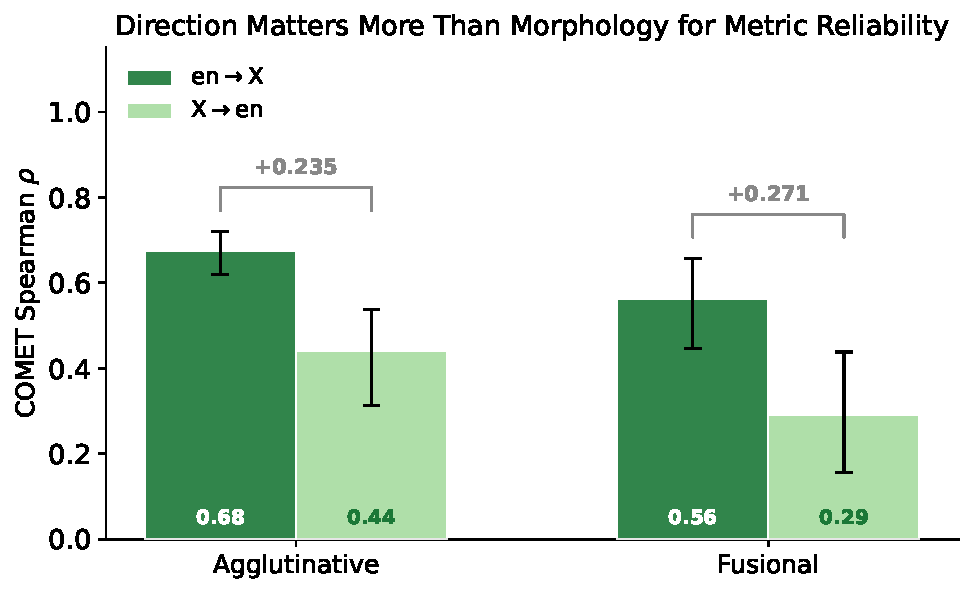
\includegraphics[width=\columnwidth]{figures/presentation_direction_morphology_teaser.pdf}
  \caption{Translation direction matters more than morphological type for COMET reliability: en$\to$X (dark green) consistently outperforms X$\to$en (light green) within both morphological types with Tier-1 data in both directions (\S\ref{sec:dir_morph}). Isolating is omitted: there are no Tier-1 en$\to$X isolating observations (Limitations), so it cannot show a direction contrast.}
  \label{fig:teaser}
\end{figure}

Automated MT metrics are the connective tissue of modern MT research: they drive model selection, benchmark comparisons, and shared-task rankings across hundreds of language pairs. Yet the conditions under which these metrics are trustworthy remain poorly understood. A practitioner evaluating a new Hindi or Swahili translation system reaches for BLEU or COMET without knowing whether those metrics bear any reliable relationship to human judgment for that language, domain, or translation direction.

The WMT Metrics Shared Task \cite{freitag2023results} has produced annual meta-evaluations for over a decade, but each edition covers only the language pairs in that year's shared task, typically 5--15 pairs, nearly always news-domain, and never with a systematic typological framing. Efforts to extend coverage to low-resource languages \cite{yari2025item} remain limited in scope. No prior work has unified professional Multidimensional Quality Metrics (MQM) annotations, crowd-sourced Direct Assessment (DA), and synthetic annotations across a common evaluation framework spanning the full range of typological diversity.

We fill this gap with AmanaMT\footnote{\emph{Amana} (Hausa, borrowed from Arabic \emph{am\=ana}): trust, reliability, honesty. Named for the benchmark's purpose: determining when and where automatic MT metrics can be trusted. Code and data: \url{https://github.com/byu-matrix-lab/amana-mt}.}, a unified three-tier benchmark across \NumLanguages\ languages, \NumMetrics\ metrics, and \TotalSegments\ segments. Our design enables the first direct comparison of metric reliability across resource tiers, translation directions, and morphological types in a single controlled study. The results reveal that the field's go-to explanation for metric failure, ``this language is low-resource,'' is often wrong in a correctable way: domain mismatch and the joint configuration of translation direction and morphological type predict failure far better than resource level alone.

\subsection{Contributions}

\textbf{Direction dominates over morphological type.} We quantify metric reliability across a 2$\times$3 grid of translation direction (en$\to$X, X$\to$en, X$\leftrightarrow$Y) and morphological type (isolating, agglutinative, fusional). Translation direction is the dominant predictor ($\eta^2_{\text{dir}}=\EtaSqDir$, nearly a third of between-language variance); morphological type is a much smaller main effect ($\eta^2_{\text{morph}}=\EtaSqMorph$). The joint direction$\times$morphology cells account for $\eta^2_{\text{cell}}=\EtaSqInteract$, capturing direction-specific morphological variation (particularly within X$\to$en) absent from prior MT meta-evaluation work.

\textbf{Domain as the primary confound.} Ukrainian's near-zero correlation ($\rho=\LangCOMETUK$) is fully explained by a domain label mismatch (\texttt{uk-en\_2022\_other}): every Ukrainian segment is conversational-register text evaluated against a news-trained metric. Controlled comparison with direction-matched X$\to$en languages confirms a $\UkJaGap$ absolute gap to the next-lowest language (ja-en), attributable to domain shift, not language difficulty.

\textbf{Simpson's Paradox in multi-year evaluation.} Russian's anomalously low aggregate correlation ($\rho=\LangCOMETRU$) conceals clean per-year signals ($\rho=\RuWmtOneRho$ in 2021, $\RuWmtTwoRho$ in 2022). Pooling WMT system generations across years creates aggregation bias that should be treated as a methodological artefact, not a linguistic finding.

\textbf{Neural metrics dominate across typological cells and resource tiers.} MetricX-24, xCOMET, and COMET outperform surface metrics in every typological cell and at every resource tier. The gap is largest for the hardest cases: morphologically complex languages and non-news domains.

%% ------------------------------------------
\section{Related Work}
\label{sec:related}

\paragraph{WMT Metrics Shared Task.}
The primary venue for systematic MT metric evaluation is the annual WMT Metrics Shared Task, which has evolved from BLEU-focused comparisons \cite{bojar2017wmt} to MQM-based meta-evaluation \cite{freitag2023results}. Each edition covers 5--15 language pairs with professional MQM annotations, generating yearly rankings. Our work differs in three ways: (1) we aggregate across years rather than evaluating a single shared-task snapshot; (2) we include 22 additional language pairs via DA and synthetic annotations; (3) we frame results typologically rather than as a ranking exercise.

\paragraph{MQM and annotation quality.}
\citet{freitag2021experts} establish that expert MQM annotation substantially outperforms crowd-sourced DA for high-quality MT evaluation. \citet{deutsch2023ties} show that tie handling in pairwise accuracy (PA) materially affects rankings, motivating our adoption of soft pairwise accuracy (SPA) \cite{thompson2024spa}. Reference quality as a confound is studied by \citet{freitag2023results}, who argue that ``metrics might be guilty but references are not innocent.''

\paragraph{Metric reliability under domain and resource shift.}
\citet{zouhar2024domain} demonstrate that learned metrics fine-tuned on WMT news data degrade substantially when applied to out-of-domain text, directly predicting the Ukrainian result we observe. \citet{yari2025item} find that metric reliability varies significantly across Indian languages, with low-resource languages showing systematically weaker correlations, a finding our broader typological framing partially confirms and partially complicates (Khmer is low-resource but correlates well due to domain homogeneity).

\paragraph{Morphology and MT evaluation.}
\citet{mondshine2025ngrams} study metric reliability across morphological types in summarization and find that COMET correlates better for fusional languages, the inverse of the sign we observe within X$\to$en. In MT, morphological type is not an independent main driver of metric reliability ($\eta^2_{\text{morph}}=\EtaSqMorph$); the direction axis, absent from monolingual summarization, dominates instead, and morphology's residual effect only surfaces as a within-direction interaction rather than a standalone predictor. \citet{bugliarello2020xmi} show that MT difficulty (cross-mutual information) is asymmetric across translation direction; we show the same asymmetry holds for metric reliability, extending their finding from difficulty to evaluability.

\paragraph{Typological diversity in NLP.}
The broader context for this work is the recognition that NLP systems, including evaluation metrics, are not language-agnostic \cite{costa2022no}. The morphological and directional effects we quantify are one instance of a general pattern: models trained predominantly on English-centric data inherit English-centric assumptions about what good translation looks like.

%% ------------------------------------------
\section{Methodology}
\label{sec:method}

\subsection{Three-Tier Annotation Design}

A core contribution is the unified three-tier data pipeline that brings together human and synthetic annotations under a shared evaluation framework:

\textbf{Tier~1a, WMT MQM} (\textit{high-resource}): Professional Multidimensional Quality Metrics span-level annotations from the WMT shared task \cite{freitag2021experts}, covering de, zh, ru, he (WMT20--23). Segment-level MQM penalty scores are converted to sentence-level quality scores via the standard weighted formula. WMT24 en-es also uses MQM annotation but is tiered as Medium, not High (see \S\ref{sec:per_lang}), since it is single-year with a more recent system generation and annotation cohort than de/zh/ru/he.

\textbf{Tier~1b, WMT Direct Assessment} (\textit{medium/low-resource}): Sentence-level DA scores from the WMT direct assessment protocol \cite{graham2017crowd} covering cs, tr, uk (medium) and ha, km, ps (low-resource), drawn from the corresponding per-year WMT shared task releases. DA scores are normalized to [0,\,1].

\label{sec:tier2}\textbf{Tier~2, Synthetic MQM} (\textit{very-low-resource}): For \NumTierTwoLanguages\ languages with no human MT annotations (sw, ht, lo, th, my, am, ka), we generate hypotheses using NLLB-200 \cite{costa2022no} over FLORES+ \cite{goyal2022flores,costa2022no} source sentences (\texttt{openlanguagedata/flores\_plus}, the community-maintained successor to FLORES-101 that also incorporates the FLORES-200 expansion introduced alongside NLLB-200), then prompt the large language model (LLM) Llama-3.1-8B-Instruct \cite{dubey2024llama3} with a GEMBA-MQM-style few-shot template \cite{kocmi2023gembamqm} to produce synthetic span-level quality judgments. \textbf{Circular-evaluation caveat}: the same Llama-3.1-8B backbone is also evaluated as the GEMBA metric. GEMBA correlations are therefore excluded from all Tier~2 analyses; only reference-based and kiwi metrics are reported for this tier. Validation against human annotation (even 200 Error Span Annotation (ESA)-annotated segments per language) would be required to confirm that Tier~2 synthetic scores reflect real translation quality rather than LLM self-consistency.

\subsection{Metrics Evaluated}

\paragraph{Lexical surface metrics.}
\textbf{BLEU} \cite{papineni2002bleu}: $n$-gram precision with brevity penalty.
\textbf{ChrF++} \cite{popovic2015chrf}: Character $n$-gram F-score with added word-unigram/bigram terms (\texttt{sacrebleu} \texttt{word\_order=2}, the chrF++ configuration); more morphology-sensitive than BLEU.

\paragraph{Embedding-based.}
\textbf{BERTScore} \cite{zhang2019bertscore}: Contextual embedding cosine similarity (mDeBERTa-v3-base).
\textbf{BLEURT} \cite{sellam2020bleurt}: Fine-tuned BERT regression on human ratings.

\paragraph{Learned regression (reference-based).}
\textbf{COMET} \cite{rei2022comet22}: Regression over source+hypothesis+reference (wmt22-comet-da).
\textbf{xCOMET} \cite{guerreiro2023xcomet}: COMET with MQM error-span detection (XCOMET-XL).
\textbf{MetricX-24} \cite{juraska2024metricx}: Google's WMT 2024 winning hybrid metric (metricx-24-hybrid-large-v2p6-bfloat16).

\paragraph{Reference-free quality estimation.}
\textbf{COMET-Kiwi} \cite{rei2022cometkiwi} (Kiwi-22): Reference-free QE using source+hypothesis only (wmt22-cometkiwi-da).
\textbf{COMET-Kiwi-23} \cite{rei2023scaling} (CK23): Larger 2023 variant (wmt23-cometkiwi-da-xl).

\paragraph{LLM-based.}
\textbf{GEMBA-MQM} \cite{kocmi2023large,kocmi2023gembamqm}: Llama-3.1-8B-Instruct \cite{dubey2024llama3} prompted with a GEMBA-MQM few-shot template to predict MQM error spans; excluded from Tier~2 analysis (see \S\ref{sec:tier2}).

\noindent\textbf{Ensemble}: Min-max normalized score average over the five neural metrics (COMET, xCOMET, MetricX-24, Kiwi-22, Kiwi-23), excluded from Tier~2.

\subsection{Translation Direction and Morphological Type Analysis}
\label{sec:dir_morph}

A central novel contribution is a 2$\times$3 cell analysis of \emph{translation direction} crossed with \emph{morphological type}, defined at the language level as follows.

\vspace{0.3em}
\noindent\textbf{Translation direction:}
\begin{description}[noitemsep,topsep=2pt]
  \item[X$\to$en] non-English source, English target (e.g.\ zh, he, uk)
  \item[en$\to$X] English source, non-English target (e.g.\ de, tr, sw)
  \item[X$\leftrightarrow$Y] neither source nor target is English; each pair is labeled by its target language (e.g.\ fr for de$\to$fr, bn for hi$\to$bn, hi for bn$\to$hi)
\end{description}
\vspace{0.3em}
\noindent\textbf{Morphological type} (standard linguistic taxonomy):
\begin{description}[noitemsep,topsep=2pt]
  \item[isolating] minimal inflection, meaning via word order (zh, th, lo, km, my)
  \item[agglutinative] transparent suffix/prefix stacking (tr, fi, et, ka, kk, sw, ja, ta, am)
  \item[fusional] multiple grammatical features fused per morpheme (de, ru, es, cs, fr, pl, uk, he, ps, bn, hi, gu, and others)
\end{description}
\vspace{0.3em}

Khmer (km) is Austroasiatic/Mon-Khmer and isolating, not agglutinative as sometimes assumed; Burmese (my) is predominantly analytic. Hausa (ha) is classified fusional here: although it has real agglutinative affixation, its Afroasiatic verbal-grade system fuses aspect, transitivity, and direction via tone and vowel apophony rather than discrete morphemes, and its typology is genuinely mixed rather than a clean fit to either category.

For each language we compute Spearman $\rho$ between each metric and human scores, yielding a $2{\times}3$ matrix of mean $\rho$ per (direction, morphology) cell. Effect sizes are reported as $\eta^2$ (proportion of variance explained), with 95\% bootstrap CIs over the languages in each cell. $\eta^2_{\text{dir}}$ and $\eta^2_{\text{morph}}$ are computed via one-way ANOVA on the per-language $\rho$ values with direction and morphological type as the respective factors. $\eta^2_{\text{cell}}$ is computed via one-way ANOVA over the six direction$\times$morphology cells and therefore measures total between-cell variance rather than a formally partitioned interaction term; it is bounded below by each main effect by construction. The informative comparison is therefore how direction dominates the main-effect decomposition ($\eta^2_{\text{dir}}$ much larger than $\eta^2_{\text{morph}}$), while the cell structure ($\eta^2_{\text{cell}}$) captures additional direction-specific morphological variation not visible in either main effect alone.

This analysis is motivated by and extends \citet{mondshine2025ngrams}, who study metric reliability across morphological types in summarization (not MT) and find that COMET correlates \emph{better} for fusional languages in their setting, treating morphology as an independent main driver. Our result does not simply reverse their sign under an added direction confound: morphology is a substantially weaker independent main driver of metric reliability in MT than direction is ($\eta^2_{\text{morph}}=\EtaSqMorph$, versus $\eta^2_{\text{dir}}=\EtaSqDir$ for direction). Their morphology-driven story does not replicate as a standalone effect in our MT setting; what residual morphological signal exists is direction-dependent (\S\ref{sec:dir_morph}), a structurally different claim from theirs. The direction axis is independently motivated by \citet{bugliarello2020xmi}, who show that translation \emph{difficulty} (measured via cross-mutual information) is asymmetric across direction; our contribution is showing the same asymmetry holds for metric \emph{reliability}.

\subsection{Evaluation Protocol}

For each (language, metric) pair, we compute:
(1) Spearman $\rho$ with 95\% bootstrap confidence intervals (1000 resamples, percentile method);
(2) Kendall $\tau$;
(3) Pairwise accuracy (PA), fraction of concordant segment pairs, excluding metric-tied and human-tied pairs \cite{freitag2023results};
(4) Soft pairwise accuracy (SPA), the WMT 2024 standard \cite{thompson2024spa}, which credits metric-tied pairs as 0.5 rather than excluding them, providing a tie-calibrated alternative to PA \cite{deutsch2023ties};
(5) Williams \citeyearpar{williams1959} test for significance of the difference between two correlations sharing a common criterion.

Segments where the human quality score is tied are excluded from both PA and SPA denominators, following \citet{deutsch2023ties}.

All main analysis runs over \TierOneTotalSegments\ professionally annotated segments across Tier~1a and Tier~1b; the \TotalSegments\ total segment count includes Tier~2 synthetic annotations, which are reported separately and flagged as exploratory.

%% ------------------------------------------
\section{Results and Analysis}
\label{sec:results}

\subsection{Main Correlation Results}

Table~\ref{tab:tier} reports per-tier Spearman $\rho$ and soft pairwise accuracy (SPA) averaged across all languages in each tier. Neural regression metrics dominate at every resource level; surface metrics degrade more sharply on Tier~1a (MQM) where human judges penalize subtle errors that $n$-gram overlap misses. Williams tests (COMET vs.\ BLEU and vs.\ chrF, per language) confirm COMET's advantage over surface metrics is statistically significant at every Tier~1 language (Tier~1a and Tier~1b) except \WilliamsTierOneExceptionLangs: Ukrainian is the domain-confound outlier discussed below, where COMET's own correlation collapses toward zero so it cannot significantly exceed anything; Zulu's COMET advantage is significant against BLEU ($p=\WilliamsZUBLEUvsCOMETPval$) but not against chrF ($p=\WilliamsZUCHRFvsCOMETPval$).

Tier~2 synthetic correlations are near-zero across all metrics, most consistent with the local LLM judge (Llama-3.1-8B) failing to produce reliable quality judgments for these low-resource, largely non-Latin-script languages, rather than with the MT metrics themselves failing. This uniform near-zero pattern does not itself distinguish which metric is more reliable for these languages, and we draw no such conclusion from it; without human validation of the synthetic judgments, we cannot separate this LLM-judge-unreliability explanation from a genuine ceiling on metric reliability at this resource level.

We explicitly ruled out a data-pipeline explanation: Tier~2's segment identifiers are shared across all seven languages (each keyed only by FLORES+ sentence index, with no per-language disambiguator), a structurally identical risk to the reference/segment-ID pipeline error affecting the he-en and en-es span-fallback pairs, discussed below (\S\ref{sec:per_lang}) and in Limitations. Independently rebuilding each language's quality scores from the raw synthetic-annotation cache and rejoining by language and segment confirms the reported Tier~2 correlations are correctly aligned, not an artifact of cross-language score bleed. We report Tier~2 for completeness, not as evidence for any typological claim.

\begin{table}[h]
\centering
\small
\setlength{\tabcolsep}{3pt}
\begin{tabular}{llccc}
\toprule
\textbf{Family} & \textbf{Metric} & \textbf{High} & \textbf{Med} & \textbf{Low} \\
 & & \multicolumn{3}{c}{\textit{Spearman $\rho$ / SPA}} \\
\midrule
\multirow{2}{*}{Lexical}
  & BLEU       & \TierBLEUHighRho{} / \TierBLEUHighSPA & \TierBLEUMedRho{} / \TierBLEUMedSPA & \TierBLEULowRho{} / \TierBLEULowSPA \\
  & ChrF       & \TierChrFHighRho{} / \TierChrFHighSPA & \TierChrFMedRho{} / \TierChrFMedSPA & \TierChrFLowRho{} / \TierChrFLowSPA \\
\midrule
\multirow{2}{*}{Embed.}
  & BERTScore  & \TierBERTScoreHighRho{} / \TierBERTScoreHighSPA & \TierBERTScoreMedRho{} / \TierBERTScoreMedSPA & \TierBERTScoreLowRho{} / \TierBERTScoreLowSPA \\
  & BLEURT     & \TierBLEURTHighRho{} / \TierBLEURTHighSPA & \TierBLEURTMedRho{} / \TierBLEURTMedSPA & \TierBLEURTLowRho{} / \TierBLEURTLowSPA \\
\midrule
\multirow{3}{*}{Regr.}
  & COMET      & \TierCOMETHighRho{} / \TierCOMETHighSPA & \TierCOMETMedRho{} / \TierCOMETMedSPA & \TierCOMETLowRho{} / \TierCOMETLowSPA \\
  & xCOMET     & \textbf{\TierxCOMETHighRho} / \textbf{\TierxCOMETHighSPA} & \TierxCOMETMedRho{} / \TierxCOMETMedSPA & \TierxCOMETLowRho{} / \TierxCOMETLowSPA \\
  & MetricX-24 & \TierMetricXHighRho{} / \TierMetricXHighSPA & \textbf{\TierMetricXMedRho} / \textbf{\TierMetricXMedSPA} & \textbf{\TierMetricXLowRho} / \textbf{\TierMetricXLowSPA} \\
\midrule
\multirow{2}{*}{QE}
  & Kiwi-22    & \TierKiwiXXIIHighRho{} / \TierKiwiXXIIHighSPA & \TierKiwiXXIIMedRho{} / \TierKiwiXXIIMedSPA & \TierKiwiXXIILowRho{} / \TierKiwiXXIILowSPA \\
  & Kiwi-23    & \TierKiwiXXIIIHighRho{} / \TierKiwiXXIIIHighSPA & \TierKiwiXXIIIMedRho{} / \TierKiwiXXIIIMedSPA & \TierKiwiXXIIILowRho{} / \TierKiwiXXIIILowSPA \\
\midrule
LLM  & GEMBA   & \TierGEMBAHighRho{} / \TierGEMBAHighSPA & -- & -- \\
\midrule
--  & Ensemble & \TierEnsembleHighRho{} / \TierEnsembleHighSPA & \TierEnsembleMedRho{} / \TierEnsembleMedSPA & \TierEnsembleLowRho{} / \TierEnsembleLowSPA \\
\bottomrule
\end{tabular}
\caption{Average Spearman $\rho$ / soft pairwise accuracy (SPA) by resource tier. High = Tier~1a MQM (de, ru, zh, he); Med = Tier~1b DA plus en-es WMT24 MQM; Low = Tier~1b DA. Values are averaged across annotation tiers within each resource tier. \textbf{Bold}: best single metric per tier. GEMBA shown for MQM tier only; excluded from Tier~1b (Med, Low) because its backbone was not fine-tuned on DA-style human judgments, and from Tier~2 to avoid circular evaluation with the Llama-3.1-8B-generated hypotheses. GEMBA's High-tier value averages only de/ru/zh, not all four Tier~1a languages: he-en's GEMBA score predates a segment-identifier correction applied to every other metric (\S\ref{sec:per_lang}) and could not be realigned, so it is excluded pending recomputation (see Limitations). en-es's GEMBA score has the same problem and is excluded from all reported statistics, but this does not affect the High-tier average shown here, since en-es is tiered Medium, not High (\S\ref{sec:per_lang}).}
\label{tab:tier}
\end{table}

\subsection{Per-Language Analysis}
\label{sec:per_lang}

Figure~\ref{fig:heatmap} shows per-language Spearman $\rho$ for COMET. Notable patterns:

\begin{figure*}[t]
  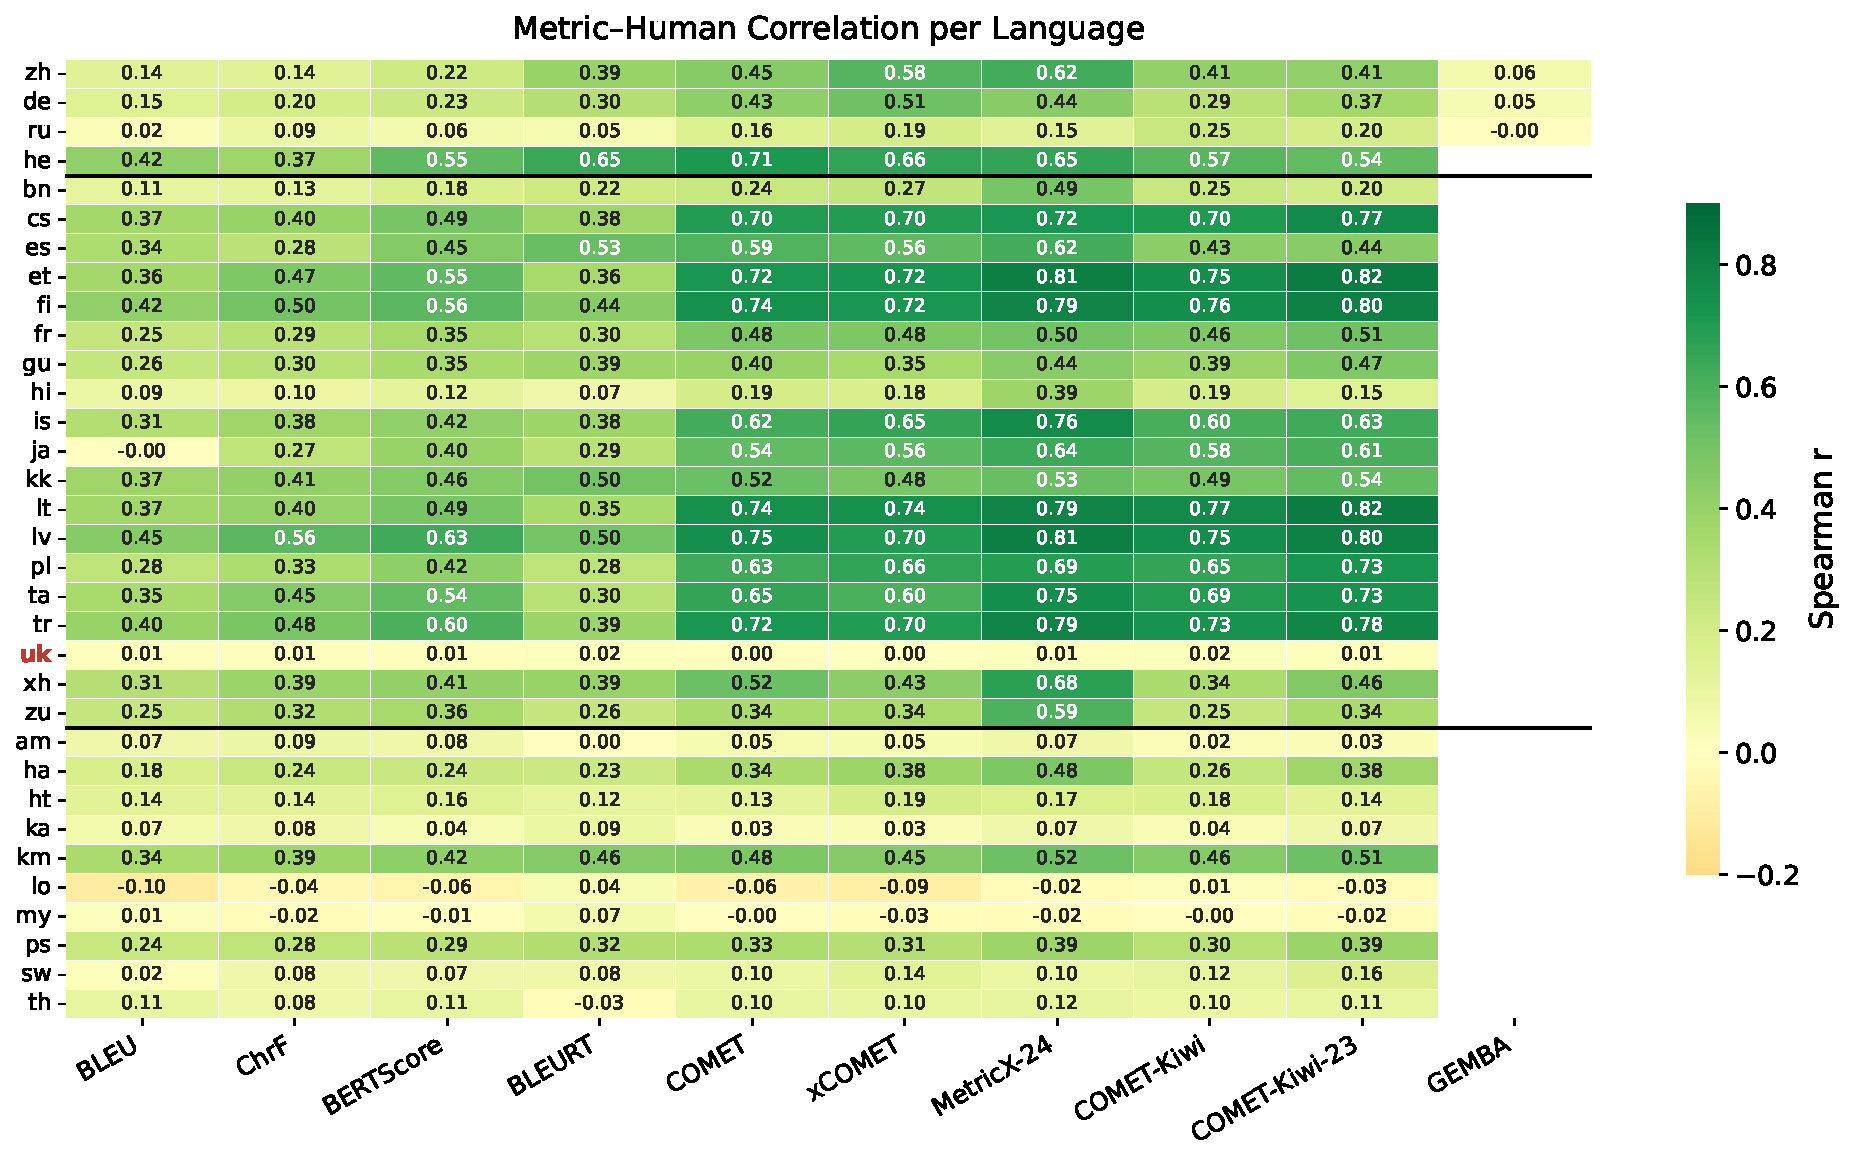
\includegraphics[width=\textwidth]{figures/presentation_language_heatmap.pdf}
  \caption{Per-language Spearman $\rho$ heatmap for all evaluated metrics. Languages sorted by resource tier. Black horizontal lines divide tiers. Ukrainian (\textbf{\textcolor{red!60!black}{uk}}) is a domain outlier (non-news register; see \S\ref{sec:per_lang}). \textit{Tier~2 languages} (am, ht, ka, lo, my, sw, th) use synthetic MQM annotations generated by Llama-3.1-8B; their correlations are exploratory and unvalidated against human judgments. GEMBA's column is sparse by design: it is reported only for the high-resource MQM languages (\S\ref{sec:tier2}), excluded from Tier~1b because its backbone was not fine-tuned on DA-style judgments, and excluded from Tier~2 to avoid circular evaluation with the Llama-3.1-8B-generated hypotheses. he-en is additionally blank for GEMBA specifically: its scores predate a segment-identifier correction applied to every other metric (\S\ref{sec:per_lang}) and could not be realigned (see Limitations).}
  \label{fig:heatmap}
\end{figure*}

\textbf{Top performers}: Latvian achieves the highest individual COMET correlation ($\rho = \LangCOMETLV$), followed by Lithuanian ($\SepCOMETLTEX$), Finnish ($\SepCOMETFIEX$), Turkish ($\SepCOMETTREX$), and Estonian ($\SepCOMETETEX$) -- all en$\to$X-specific values for the languages with data in both directions (Table~\ref{tab:dir_sep}), not the direction-pooled averages, which would understate them -- spanning two morphological types. The unifying feature is not morphological type but data quality: all five use single-year WMT DA news data with high inter-annotator agreement, suppressing the multi-year pooling variance that depresses Russian and German.

\textbf{Ukrainian} collapses to near-zero correlation for all metrics ($\rho_{\text{COMET}} = \LangCOMETUK$, pairwise acc.\ $= \LangUKCOMETPairwiseAcc$). A uniform near-zero result across unrelated metric families (surface overlap and learned regression alike) is also the signature of a broken human-score join, so before accepting a domain explanation we independently rebuilt Ukrainian's quality scores from the raw WMT DA data and rejoined them to every metric checkpoint by segment ID: the alignment is correct, and the near-zero result is not a pipeline artifact. Investigation confirmed the cause: all \LangNUK\ Ukrainian segments in the WMT DA dataset carry the domain label \texttt{other} (segment IDs: \texttt{uk-en\_2022\_other}), indicating non-news text, whereas every other language in our pipeline uses news-domain test sets. The short average sentence length ($\approx$12 words) is consistent with a conversational or social-media register \cite{kocmi2024findings}. A single-reference metric evaluated against conversational MT cannot discriminate quality adequately. Ukrainian should be treated as a domain outlier, not a language/script effect, consistent with \citet{zouhar2024domain}, who show that fine-tuned metrics degrade substantially under domain shift. We applied the same segment-ID rebuild-and-rejoin check to is-en and ha-en, the two other languages with weak aggregate correlations (Table~\ref{tab:dir_sep}); both alignments are correct, and their weakness is annotation noise rather than a domain or pipeline effect.

\textbf{Medium $>$ High}: Averaged across metrics, medium-resource languages outperform high-resource (COMET: $\rho=\TierCOMETMedRho$ vs.\ $\TierCOMETHighRho$; MetricX: $\TierMetricXMedRho$ vs.\ $\TierMetricXHighRho$; Figure~\ref{fig:tierbar} plots this for all ten metrics). This reverses the intuitive ordering and mirrors the Hindi anomaly reported by \citet{yari2025item} in Indian-language MT evaluation. The mechanistic explanation is that high-resource MQM languages span multiple WMT years (2020--23) and MT systems, introducing inter-year domain and system variance that suppresses aggregate correlation, a source of noise absent from the medium-tier DA languages.

Spanish (en-es WMT24) is classified in the medium tier despite using MQM annotation because it comes from a single year with a more recent system generation and annotation cohort. Had it been grouped with High, the medium$>$high gap would be smaller, not larger: High would rise from $\TierCOMETHighRho$ to approximately $\TierCOMETHighPlusEsRho$, and removing Spanish from Medium would lower the medium-tier mean; the ordering survives but with a narrower margin.

\textbf{Russian anomaly, Simpson's Paradox}: Russian achieves the lowest MQM correlation of any non-domain-outlier language (aggregate COMET $\rho=\LangCOMETRU$). Year-stratified analysis reveals the mechanism: WMT21-only yields $\rho=\RuWmtOneRho$ ($n=\RuWmtOneN$) and WMT22-only yields $\rho=\RuWmtTwoRho$ ($n=\RuWmtTwoN$), but pooling both years collapses to $\LangCOMETRU$. This is a textbook aggregation bias: the two WMT system pools have different quality distributions, so across-year pooling creates a between-year confound that suppresses the within-year metric--human relationship. German shows the same pattern but less severely (2020: $\rho=\DeWmtTwoZeroRho$; 2021: $\DeWmtTwoOneRho$; 2022: $\DeWmtTwoTwoRho$; aggregate: $\LangCOMETDE$). The Russian aggregate is extreme because its two yearly pools are more divergent. This is not a property of Russian as a language, it is an artefact of pooling heterogeneous MT system generations.

\textbf{Khmer}: Despite being classified as low-resource, Khmer achieves COMET $\rho=\LangCOMETKM$ and MetricX $\rho=\LangMetricXKM$, higher than several medium-tier languages (e.g., Japanese $\LangCOMETJA$, Hindi $\LangCOMETHI$). Khmer is Austroasiatic (Mon-Khmer) and typologically \emph{isolating} (not agglutinative as sometimes assumed), sharing that property with Chinese and Thai. Its strong performance here reflects single-year Wikipedia-domain data, which produces cleaner and more consistently-structured reference translations than news. This suggests that annotation consistency and domain homogeneity can compensate for low absolute resource level.

\textbf{Hebrew} shows no metric-family anomaly: COMET (reference-based) achieves the strongest correlation of any metric reported for this language ($\rho=\LangCOMETHE$), ahead of xCOMET ($\rho=\LangXCOMETHE$), MetricX ($\rho=\LangMetricXHE$), CK23 ($\rho=\LangKiwiXXIIIHE$), COMET-Kiwi-22 ($\rho=\LangKiwiHE$), and BERTScore ($\rho=\LangBERTScoreHE$), despite Hebrew having \LangNHE\ professionally annotated segments. Figure~\ref{fig:kiwi_scatter} shows this COMET-over-CK23 gap is the largest deviation from the reference-free/reference-based equal-performance diagonal across all evaluated languages. An earlier version of this analysis reported the reverse pattern (reference-based COMET substantially underperforming reference-free QE) and attributed it to Hebrew being out-of-distribution for COMET-22's training window. That result traced to a reference-omission error in the data-loading pipeline for the he-en span-fallback pair (see Limitations), not to a property of the metric or the language; correcting it reverses the finding. We validated the correction externally, not just internally, and at segment level rather than system level: aggregating to one mean per system before correlating (as an earlier draft did) is a weak check, since averaging cancels exactly the kind of per-segment misalignment this correction fixes. For both affected language pairs (he-en, en-es) and all four affected metrics (COMET, BLEURT, xCOMET, MetricX), we paired our corrected per-segment scores directly against the official \texttt{mt-metrics-eval-v2} \citep{freitag2023results} per-(system, segment) baseline releases for WMT23 he-en and WMT24 en-es, across all \BaselineValNChecks\ (language, metric) checks ($n\approx$8,700--8,900 segment pairs each). COMET and xCOMET, whose checkpoints match the official baseline exactly (\texttt{wmt22-comet-da}, \texttt{XCOMET-XL}), agree closely with the official scores (Pearson/Spearman $r\geq\BaselineValCoreMinPearson$/$\BaselineValCoreMinSpearman$). BLEURT and MetricX agree more weakly overall (Pearson/Spearman $r\geq\BaselineValMinPearson$/$\BaselineValMinSpearman$), which traces to a genuine checkpoint-version mismatch rather than a residual alignment error: we score BLEURT with an unofficial HF port (\texttt{Elron/bleurt-large-512}) rather than Google's official \texttt{BLEURT-20} checkpoint, and for he-en specifically the official WMT23 baseline is \texttt{MetricX-23} while our pipeline scores every language with the newer \texttt{MetricX-24}.

\begin{figure*}[t]
  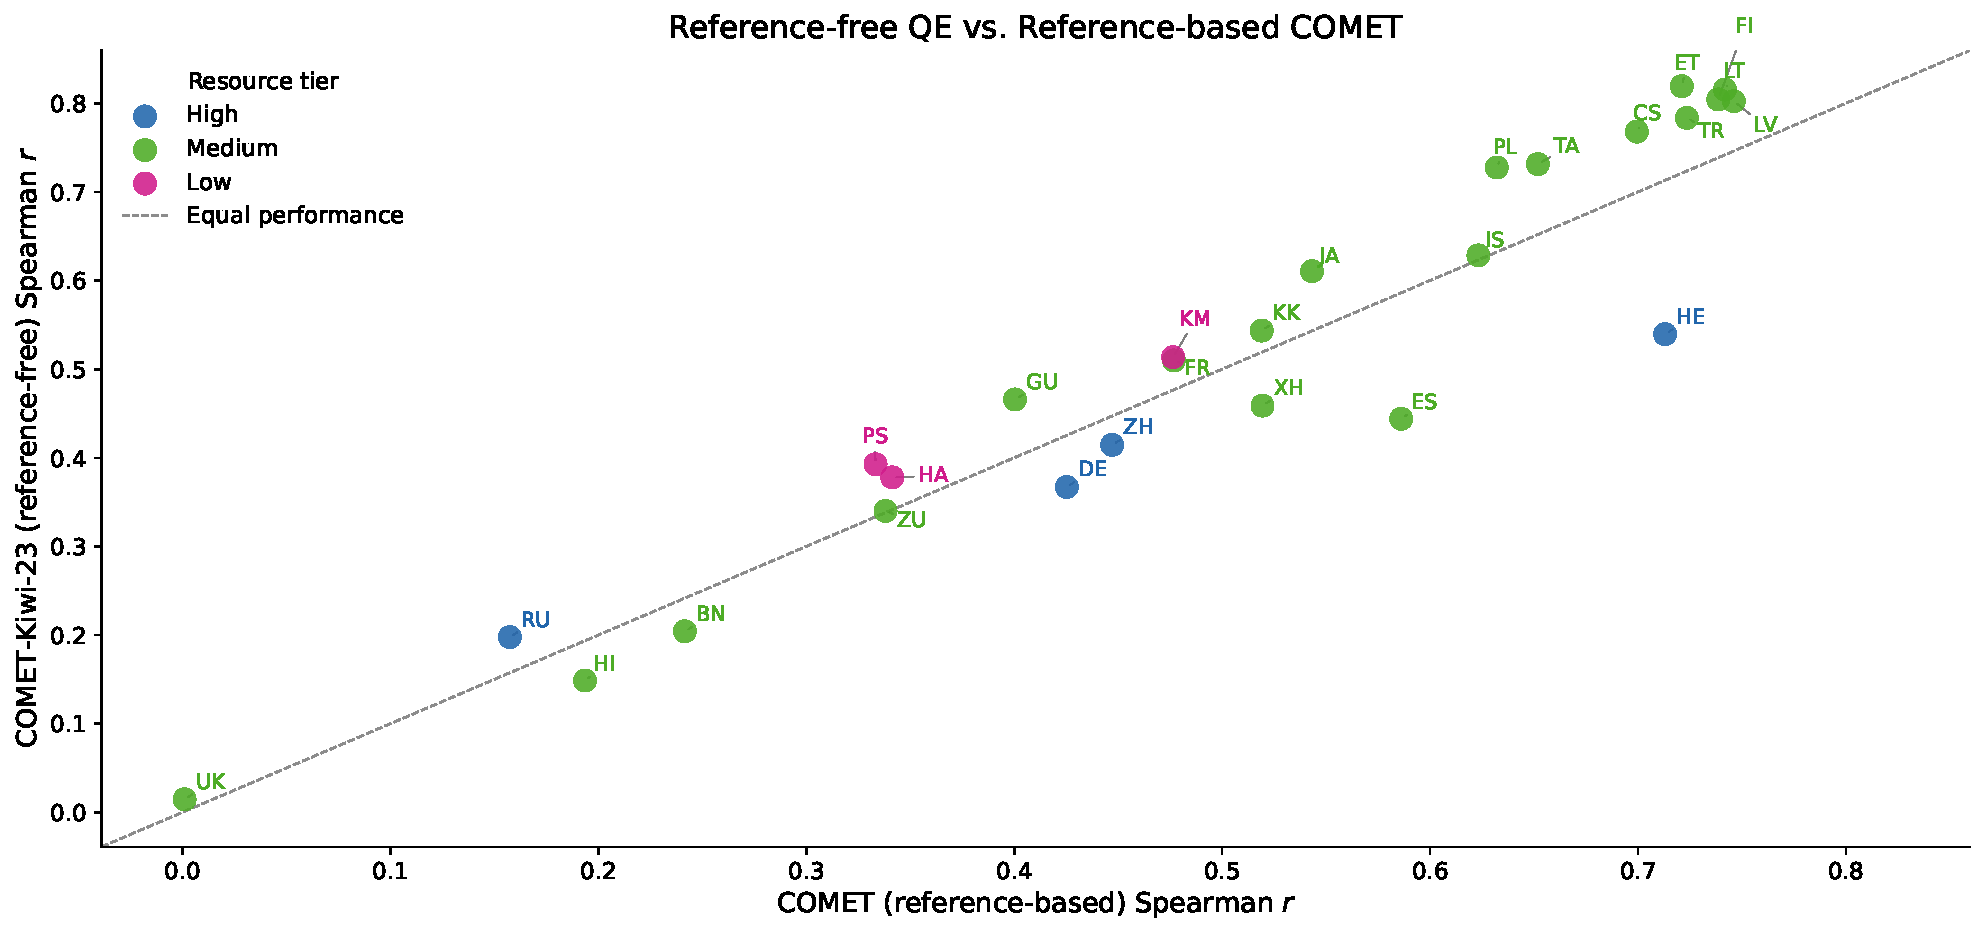
\includegraphics[width=\textwidth]{figures/presentation_kiwi23_vs_comet.pdf}
  \caption{CK23 (reference-free) vs.\ COMET (reference-based) Spearman $\rho$ for all \NumHumanAnnotatedLanguages\ languages with human annotations. Most languages cluster near the equal-performance diagonal, with reference-free QE holding a modest overall edge. Hebrew and Spanish are the two largest deviations from the diagonal in the dataset, both in COMET's favor ($\GapHeKiwiComet$ and $\GapEsKiwiComet$ Spearman points, CK23 minus COMET); we have no validated explanation for either and do not speculate one. uk sits below the diagonal for both metrics due to domain mismatch (see \S\ref{sec:per_lang}); ru reflects a Simpson's Paradox aggregate.}
  \label{fig:kiwi_scatter}
\end{figure*}

\textbf{Spanish} (WMT24 en-es) achieves the strongest correlations of any MQM language: MetricX $\rho=\LangMetricXES$, COMET $\rho=\LangCOMETES$. Classified in the medium tier (single-year, recent system generation), it is consistent with en$\to$es being the most resource-rich, morphologically regular fusional en$\to$X pair in the benchmark: alphabetic script, abundant training data, and single-year WMT24 annotations with high inter-annotator agreement.
Spanish confirms the upper bound of what learned metrics can achieve on well-matched conditions.

\begin{figure*}[t]
  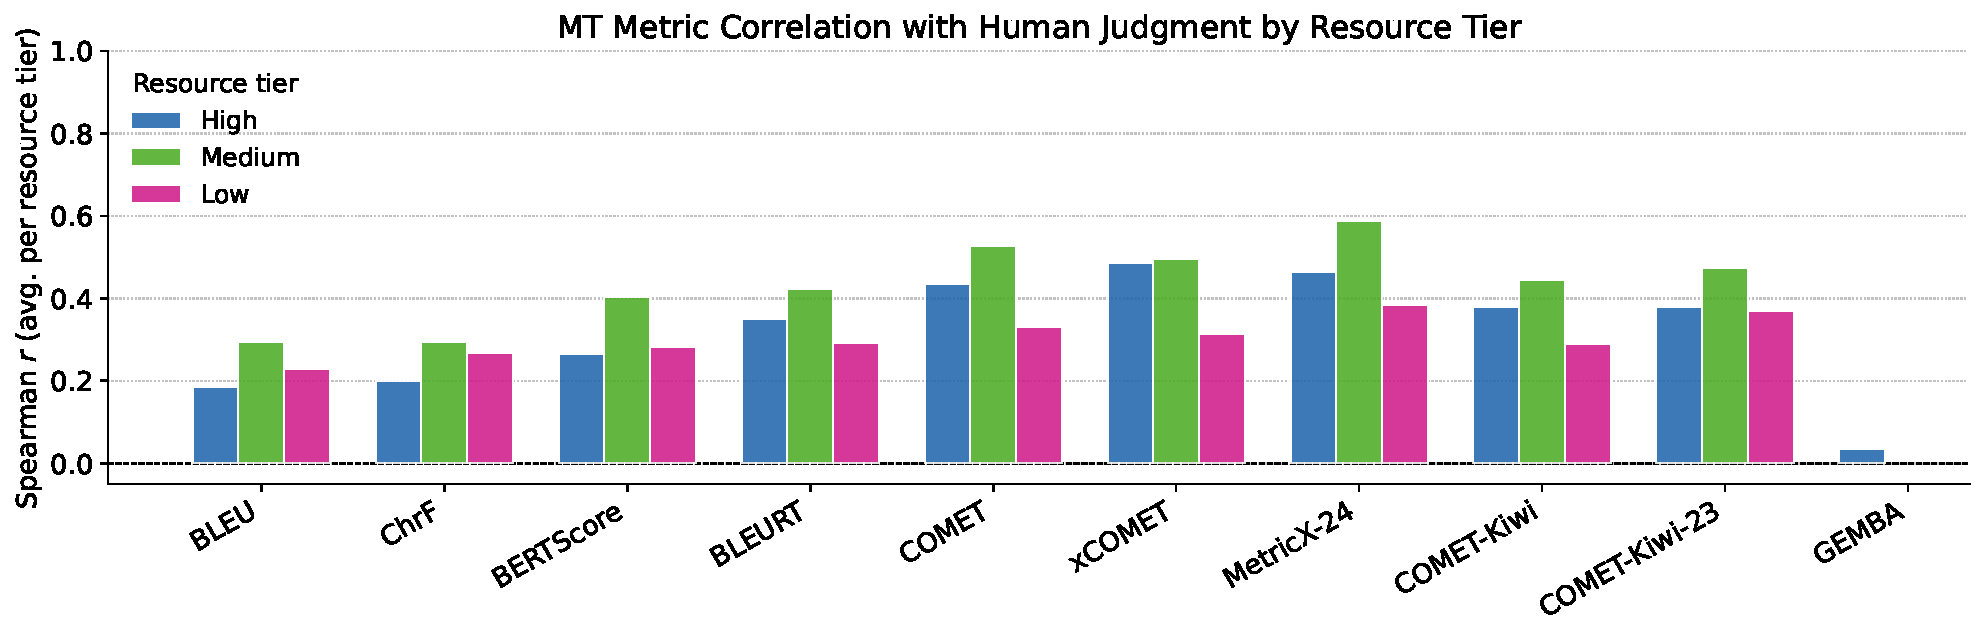
\includegraphics[width=\textwidth]{figures/presentation_tier_bar.pdf}
  \caption{Average Spearman $\rho$ by metric and resource tier. The medium $>$ high anomaly holds for all ten metrics with a Medium-tier value (GEMBA has none, excluded from Tier~1b by design: Table~\ref{tab:tier}); it is explained by cross-year pooling variance in the high-resource MQM tier (see \S\ref{sec:per_lang}).}
  \label{fig:tierbar}
\end{figure*}

\subsection{Statistical Robustness}

Bootstrap 95\% CIs are narrow for large-corpus languages (de COMET: $[\LangCOMETDECIlo, \LangCOMETDECIhi]$, $n=\LangNDE$) and wider for small ones (ps COMET: $[\LangCOMETPSCIlo, \LangCOMETPSCIhi]$, $n=\LangNPS$), confirming that high-confidence claims require $n \gtrsim 10{,}000$ segments. All Tier~1a and Tier~1b COMET correlations except Ukrainian are significant at $p < 10^{-10}$ or better. Ukrainian COMET $p = \LangUKCOMETPval$ (domain outlier). Russian despite $n=\LangNRU$ achieves $p \ll 10^{-10}$, but $\rho=\LangCOMETRU$, statistically significant but practically weak, highlighting that statistical significance and practical reliability are distinct in large-$n$ meta-evaluation.

\subsection{Translation Direction $\times$ Morphological Type}

Table~\ref{tab:dir_morph} reports the 2$\times$3 cell means for COMET (full results across all ten metrics are in the released code and data repository). \NumMixedLangs\ languages contribute data in both translation directions; we separate them by segment-id prefix before computing cell means (per-language breakdowns in Table~\ref{tab:dir_sep}). The dominant pattern is directional: en$\to$X languages score substantially above X$\to$en across both morphological types.
\begin{itemize}
  \item \textbf{Agglutinative:} en$\to$X $\rho=\DirMorphCOMETEntoXAgglutin$ vs.\ X$\to$en $\rho=\DirMorphCOMETXtoEnAgglutin$, a gap of $+\GapDirAgglutin$.
  \item \textbf{Fusional:} en$\to$X $\rho=\DirMorphCOMETEntoXFusional$ vs.\ X$\to$en $\rho=\DirMorphCOMETXtoEnFusional$ (depressed by the Ukrainian domain outlier, included here for transparency rather than excluded), a gap of $+\GapDirFusional$.
\end{itemize}
The difference-in-differences between the fusional direction gap and the agglutinative direction gap is $\DiDValue$ (Table~\ref{tab:dir_morph}), indicating the direction effect is largely constant across morphological types with only a modest interaction. The best metric varies by direction: CK23 leads X$\to$en while MetricX leads en$\to$X in \WinEntoXAgglutin\ of \WinTotalEntoXAgglutin\ agglutinative languages.

\paragraph{Robustness: mixed-effects model.} The one-way ANOVAs above treat every (language, direction) row as independent, but \NumMixedLangs\ languages contribute two correlated rows each (one per direction). To check whether this affects the conclusions, we fit a linear mixed-effects model via restricted maximum likelihood (REML): $\rho \sim$ direction + morphology, random intercept per language, $n=\MixedModelNObs$ observations, $\MixedModelNLangs$ languages. Direction remains highly significant (X$\to$en coefficient $\MixedModelDirXtoEnCoef$, $p=\MixedModelDirXtoEnP$); the fusional-vs-agglutinative morphology coefficient does not reach significance ($\MixedModelMorphFusionalCoef$, $p=\MixedModelMorphFusionalP$). The language random intercept absorbs $\MixedModelICC$ of total variance (the intraclass correlation, ICC), confirming the non-independence this model was designed to check for. The mixed-effects model agrees with the ANOVA: morphological type is not an independently detectable main effect once repeated-measures structure is modeled explicitly, and direction remains the dominant, robustly significant predictor.

\paragraph{Robustness: year stratification.} Only de, ru, zh, and cs are multi-year in this cell analysis; every other contributing language is single-year. de and ru enter the en$\to$X$\times$fusional cell via their pooled (not year-stratified) rho, and \S\ref{sec:domain_confound} already shows ru's pooled value is Simpson's-Paradox-suppressed. Substituting each language's mean-of-per-year rho for its pooled value moves that cell's mean from $\YearStratEntoXFusionalPooled$ to $\YearStratEntoXFusionalStrat$, a small increase, meaning year-stratification if anything slightly strengthens the en$\to$X advantage rather than explaining it away. A fully rigorous per-metric training-coverage control (checking whether each metric's training-data volume differs by direction) is not attempted here: none of the \NumMetrics\ metrics publish per-language-pair-and-direction training coverage at the granularity this would require, and we flag it as future work.

\begin{table}[t]
\centering
\small
\setlength{\tabcolsep}{3pt}
\begin{tabular}{lccc}
\toprule
\textbf{Dir.} & \textbf{Isol.} & \textbf{Agglutin.} & \textbf{Fusional} \\
 & \multicolumn{3}{c}{\textit{Mean COMET $\rho$ [95\% CI]}} \\
\midrule
X$\to$en  & \DirMorphCOMETXtoEnIsolating{} [---] & \textbf{\DirMorphCOMETXtoEnAgglutin}{\scriptsize[\DirMorphCOMETXtoEnAgglutinCIlo,\DirMorphCOMETXtoEnAgglutinCIhi]} & \DirMorphCOMETXtoEnFusional{}{\scriptsize[\DirMorphCOMETXtoEnFusionalCIlo,\DirMorphCOMETXtoEnFusionalCIhi]} \\
en$\to$X  & --            & \DirMorphCOMETEntoXAgglutin{}{\scriptsize[\DirMorphCOMETEntoXAgglutinCIlo,\DirMorphCOMETEntoXAgglutinCIhi]} & \DirMorphCOMETEntoXFusional{}{\scriptsize[\DirMorphCOMETEntoXFusionalCIlo,\DirMorphCOMETEntoXFusionalCIhi]} \\
X$\leftrightarrow$Y      & --            & --                 & \DirMorphCOMETPivotFusional{}{\scriptsize[\DirMorphCOMETPivotFusionalCIlo,\DirMorphCOMETPivotFusionalCIhi]} \\
\midrule
$\eta^2_{\text{dir}}$ & \multicolumn{3}{c}{\EtaSqDir} \\
$\eta^2_{\text{morph}}$ & \multicolumn{3}{c}{\EtaSqMorph} \\
$\eta^2_{\text{cell}}$ & \multicolumn{3}{c}{\EtaSqInteract} \\
\bottomrule
\end{tabular}
\caption{Mean COMET Spearman $\rho$ by translation direction and morphological type. Cells with $n{\le}2$ languages have no CI (marked [---]). Empty (--) = no Tier-1 languages in that cell. $\eta^2$ via one-way ANOVA on per-language $\rho$. Russian ($\rho=\LangCOMETRU$, en$\to$X+fusional) and Ukrainian ($\rho=\LangCOMETUK$, X$\to$en+fusional) are included in their cells; see \S\ref{sec:per_lang}. \textbf{Bold} marks the X$\to$en agglutinative cell specifically because it is where the reference-free metric CK23 (not shown in this COMET-only table) wins all \WinXtoEnAgglutin/\WinTotalXtoEnAgglutin\ direction-separated pairs (Table~\ref{tab:dir_sep}); no other cell in this table carries that meaning, and $\eta^2$ values below are never bolded.}
\label{tab:dir_morph}
\end{table}

\begin{table}[h]
\centering
\small
\setlength{\tabcolsep}{1pt}
\begin{tabular}{lccccc}
\toprule
\textbf{Direction} & \textbf{BLEU} & \textbf{ChrF++} & \textbf{COMET} & \textbf{xCOMET} & \textbf{MetricX} \\
\midrule
en$\to$X  & \DirMetricBLEUEntoX & \DirMetricChrFEntoX & \DirMetricCOMETEntoX & \DirMetricxCOMETEntoX & \textbf{\DirMetricMetricXEntoX} \\
X$\to$en  & \DirMetricBLEUXtoEn & \DirMetricChrFXtoEn & \DirMetricCOMETXtoEn & \DirMetricxCOMETXtoEn & \textbf{\DirMetricMetricXXtoEn} \\
X$\leftrightarrow$Y      & \DirMetricBLEUPivot & \DirMetricChrFPivot & \DirMetricCOMETPivot & \DirMetricxCOMETPivot & \textbf{\DirMetricMetricXPivot} \\
\bottomrule
\end{tabular}
\caption{Mean Spearman $\rho$ by translation direction for five representative metrics (averaged across all languages in each direction group). MetricX-24 leads across all three directions among these five metrics, including X$\to$en, where it now edges out CK23 (not shown) by a narrow margin ($\rho{=}\DirMetricMetricXXtoEn$ vs.\ $\rho{=}\DirMetricCKXXIIIXtoEn$); this pooled ranking is not the same question as which metric wins the most individual X$\to$en language pairs (Table~\ref{tab:lookup}), where CK23 remains the more frequent winner. X$\leftrightarrow$Y pairs show the lowest surface-metric scores but near-parity on MetricX.}
\label{tab:dir_metric}
\end{table}

Contrast with \citet{mondshine2025ngrams}: in their summarization setting, COMET correlates \emph{better} for fusional languages (coherence Pearson $\approx 0.35$ for high-fusional vs.\ $0.07$ for isolating). In the MT setting the dominant factor is direction, not morphological type: fusional X$\to$en languages score only $\rho=\DirMorphCOMETXtoEnFusional$ (depressed by the Ukrainian outlier), while fusional en$\to$X languages score $\rho=\DirMorphCOMETEntoXFusional$, a gap of $+\GapDirFusional$ attributable to translation direction. Agglutinative languages show the same directional pattern ($\rho=\DirMorphCOMETXtoEnAgglutin$ X$\to$en vs.\ $\rho=\DirMorphCOMETEntoXAgglutin$ en$\to$X, a gap of $+\GapDirAgglutin$), confirming that direction dominates in the MT setting: within this design we cannot detect an independent morphological main effect (the empty en$\to$X isolating cell limits what the data can rule out; see Limitations). $\eta^2_{\text{cell}}=\EtaSqInteract$ quantifies the combined effect; $\eta^2_{\text{dir}}=\EtaSqDir$ isolates direction as the dominant contributor.

\subsection{Typological Predictors of Metric Choice}
\label{sec:predictor}

Translation direction is the dominant predictor of metric reliability ($\eta^2_{\text{dir}}=\EtaSqDir$; \S\ref{sec:dir_morph}); we now ask whether that directional signal extends to metric \emph{choice}, that is, which metric a practitioner should prefer for an unseen language.

For each of the \NumHumanAnnotatedLanguages\ languages with human annotations, we rank all metrics by Spearman $\rho$ and record the best-performing metric.
Table~\ref{tab:lookup} summarizes these \TableFourTotalPairs\ direction-language pair observations (\TableFourMainPipelinePairs\ in the main pipeline; de-en held out as a blind validation), with leave-one-out (LOO) cross-validation for cells with $n \geq 6$ (overall \LOOOverallCorrect/\LOOOverallTotal\ = \LOOOverallPct\%). Isolating X$\to$en ($n{=}\WinTotalXtoEnIsolating$) and X$\leftrightarrow$Y ($n{=}\PivotN$) fall below this threshold and are marked `--' in the LOO column rather than validated.
The most robust pattern in the table needs no morphological breakdown at all: CK23 beats COMET in all \BeatsCometEntoXAgglutin\ of \WinTotalEntoXAgglutin\ agglutinative and \BeatsCometEntoXFusional\ of \WinTotalEntoXFusional\ fusional en$\to$X pairs (\BeatsCometEntoXTotal/\EntoXTotalPairs\ overall), both cells with bootstrap CI $[\CellCIEntoXAgglutinLo, \CellCIEntoXAgglutinHi]$ on the win fraction. Table~\ref{tab:lookup} is organized first by direction, the dominant factor, and then by morphological type within each direction as a secondary refinement: even though morphology explains substantially less of the aggregate variance in reliability than direction does ($\eta^2_{\text{morph}}=\EtaSqMorph$ vs.\ $\eta^2_{\text{dir}}=\EtaSqDir$), the within-direction agglutinative-vs-fusional splits are large enough to flip which specific metric wins the discrete argmax comparison (\S\ref{sec:dir_morph}), so morphology remains a useful secondary key for the practitioner-facing recommendation even though it is not the primary driver of reliability.
Three patterns emerge:

\begin{enumerate}[leftmargin=*,itemsep=4pt,topsep=4pt]
  \item \textbf{X$\to$en: CK23 wins consistently across morphological types.} CK23 is the best metric for agglutinative X$\to$en (\WinXtoEnAgglutin/\WinTotalXtoEnAgglutin, LOO \LOOXtoEnAgglutin/\LOOTotalXtoEnAgglutin; bootstrap CI on CK23$>$COMET: $[\CellCIXtoEnAgglutinLo, \CellCIXtoEnAgglutinHi]$) and fusional X$\to$en (\WinXtoEnFusional/\WinTotalXtoEnFusional{} including Hebrew and de-en held-out, LOO \LOOXtoEnFusional/\LOOTotalXtoEnFusional{} over the smaller DA-pipeline-only subset; see Table~\ref{tab:lookup}'s note). De-en (German$\to$English, $n{=}\DeEnN$) is genuinely unseen, German enters the pipeline via WMT MQM en$\to$de only; CK23 achieves $\rho{=}\DeEnKiwiRho$ vs.\ COMET $\rho{=}\DeEnCOMETRho$ and MetricX $\rho{=}\DeEnMetricXRho$, confirming the prediction. The reference-free design sidesteps the $n$-gram overlap problem that BLEU and ChrF++ face when rich morphology produces sparse token matches.

  \item \textbf{en$\to$X: MetricX competitive for agglutinative; CK23 leads for fusional.} For agglutinative en$\to$X (\WinTotalEntoXAgglutin{} languages), MetricX wins \WinEntoXAgglutin/\WinTotalEntoXAgglutin{} (LOO \LOOEntoXAgglutin/\LOOTotalEntoXAgglutin), though margins are often small (kk: MetricX $\SepMXKKEX$ vs.\ CK23 $\SepCKXXIIIKKEX$; tr: $\SepMXTREX$ vs.\ $\SepCKXXIIITREX$). CK23 still beats COMET in \BeatsCometEntoXAgglutin/\WinTotalEntoXAgglutin{} agglutinative en$\to$X pairs (bootstrap CI $[\CellCIEntoXAgglutinLo, \CellCIEntoXAgglutinHi]$), so the CK23-vs-COMET choice is unambiguous; the MetricX advantage only matters when choosing between all three neural metrics. For fusional en$\to$X (\WinTotalEntoXFusional{} languages), CK23 wins \WinEntoXFusional/\WinTotalEntoXFusional{} and beats COMET in \BeatsCometEntoXFusional/\WinTotalEntoXFusional{} (CI $[\CellCIEntoXFusionalLo, \CellCIEntoXFusionalHi]$).

  \item \textbf{Isolating X$\to$en and X$\leftrightarrow$Y: MetricX.} MetricX-24 wins both isolating X$\to$en cases (zh: $+\GapZHMetricXBleu$ over BLEU; km: $+\GapKMMetricXBleu$; average $+\TableFourXtoEnIsolating$) and dominates X$\leftrightarrow$Y pairs (\PivotMetricXWins/\PivotN), where neither source nor target is English and reference-free QE encoders are off-domain.
\end{enumerate}

Across all profiles, the gain over BLEU from choosing the recommended metric ranges from $+\TableFourXtoEnFusional$ to $+\TableFourEntoXAgglutin$ Spearman $\rho$ (Table~\ref{tab:lookup}), the ``always use a neural metric'' message is robust even where the \emph{choice} among neural metrics is uncertain.

\begin{table*}[t]
\centering
\small
\setlength{\tabcolsep}{6pt}
\begin{tabular}{llcllc}
\toprule
\textbf{Direction} & \textbf{Morphological type} & \textbf{$n$ pairs} & \textbf{Recommended metric} & \textbf{LOO accuracy} & \textbf{Avg $\Delta\rho$ vs.\ BLEU} \\
\midrule
X$\to$en & Agglutinative & \WinTotalXtoEnAgglutin   & CometKiwi-23 (\WinXtoEnAgglutin/\WinTotalXtoEnAgglutin)          & \LOOXtoEnAgglutin/\LOOTotalXtoEnAgglutin & $+\TableFourXtoEnAgglutin$ \\
X$\to$en & Isolating     & \WinTotalXtoEnIsolating   & MetricX-24 (\WinXtoEnIsolating/\WinTotalXtoEnIsolating)            & --  & $+\TableFourXtoEnIsolating$ \\
X$\to$en & Fusional      & \WinTotalXtoEnFusional$^\dagger$ & CometKiwi-23 (\WinXtoEnFusional/\WinTotalXtoEnFusional)   & \LOOXtoEnFusional/\LOOTotalXtoEnFusional & $+\TableFourXtoEnFusional$ \\
en$\to$X & Agglutinative & \WinTotalEntoXAgglutin   & MetricX-24 (\WinEntoXAgglutin/\WinTotalEntoXAgglutin)$^\ddagger$  & \LOOEntoXAgglutin/\LOOTotalEntoXAgglutin & $+\TableFourEntoXAgglutin$ \\
en$\to$X & Fusional      & \WinTotalEntoXFusional   & CometKiwi-23 (\WinEntoXFusional/\WinTotalEntoXFusional)          & \LOOEntoXFusional/\LOOTotalEntoXFusional & $+\TableFourEntoXFusional$ \\
X$\leftrightarrow$Y & Fusional      & \PivotN   & MetricX-24 (\PivotMetricXWins/\PivotN)            & --  & $+\TableFourPivotFusional$ \\
\bottomrule
\end{tabular}
\caption{\textbf{Typological metric selection guide}: empirically observed best metric per profile across \TableFourTotalPairs\ direction-language pair observations (de-en held out). $n$ = number of direction-separated pairs; LOO accuracy = leave-one-out cross-validation (-- = cell too small to validate); Avg $\Delta\rho$ = mean Spearman gain over BLEU. $^\dagger$Fusional X$\to$en's $n{=}\WinTotalXtoEnFusional$ includes Hebrew and the held-out de-en pair, neither scored by the DA direction-separated pipeline the LOO cross-validation runs over; its LOO column (\LOOXtoEnFusional/\LOOTotalXtoEnFusional) therefore validates only the \LOOTotalXtoEnFusional\ DA-pipeline languages, a smaller denominator than the win count. Held-out de-en ($n{=}\DeEnN$, absent from main pipeline): CometKiwi-23 $\rho{=}\DeEnKiwiRho$ vs.\ COMET $\rho{=}\DeEnCOMETRho$, confirming prediction. $^\ddagger$Agglutinative en$\to$X: MetricX-24 wins \WinEntoXAgglutin/\WinTotalEntoXAgglutin, but CometKiwi-23 beats COMET in \BeatsCometEntoXAgglutin/\WinTotalEntoXAgglutin{} (bootstrap CI $[\CellCIEntoXAgglutinLo,\CellCIEntoXAgglutinHi]$); advantage often $<\KkTrMaxMargin$ $\rho$ (kk, tr).}
\label{tab:lookup}
\end{table*}

As a post-hoc check, we trained a Ridge regression predictor (World Atlas of Language Structures \citep[WALS;][]{wals} typological features + morphological type + direction, leave-one-language-out cross-validation (LOLO-CV), $n{=}\RidgeNLangs$ Tier-1 languages). Pearson $r=\RidgeCKXXIIIPearson$ for CK23 and $r=\RidgeCKPearson$ for Kiwi-22; recommendation accuracy is \RidgeRecAcc, too low to treat the predictor as deployable. The moderate $r$ for the CK family confirms that direction and CK advantage are partially co-predictable from typological features, but the low recommendation accuracy is a negative result on the stronger claim that typological features alone suffice to select among neural metrics.

%% ------------------------------------------
\section{Discussion}
\label{sec:discussion}

\subsection{The Neural-Surface Gap Scales With Morphological Complexity}

This is a claim about a different quantity than \S\ref{sec:dir_morph}: $\eta^2_{\text{morph}}=\EtaSqMorph$ measures how much morphological type explains variance in absolute metric--human correlation, and it is small. The finding here concerns the \emph{gap} between neural and surface metrics, a derived quantity that morphology predicts much more strongly than it predicts either metric's raw reliability. COMET, xCOMET, and MetricX-24 dominate at every tier and in every typological cell (Tables~\ref{tab:tier}--\ref{tab:dir_metric}), but that gap over surface metrics is not uniform: it is largest for morphologically complex languages and non-news domains, precisely the conditions where evaluation is most needed and most difficult.

For fusional X$\to$en languages (excluding the Ukrainian outlier), the COMET--BLEU gap averages $\GapCometBleuFusionalXtoEn$ Spearman points; holding direction fixed, agglutinative X$\to$en languages show a larger gap still, $\GapCometBleuAgglutinXtoEn$ (the same pattern holds en$\to$X, where the gap is $\GapCometBleuAgglutinEntoX$ for agglutinative languages). This is not simply a ceiling artifact of agglutinative X$\to$en being an easier cell overall: within X$\to$en, BLEU's own reliability is nearly flat across morphological type ($\rho\approx\DirMetricBLEUXtoEn$ pooled; agglutinative and fusional differ by only a few points), while COMET's reliability rises substantially from fusional to agglutinative. The widening gap comes from COMET tracking something morphology-related that BLEU does not, not from BLEU degrading uniformly.

This is consistent with $n$-gram overlap systematically underestimating adequacy when target morphology is rich: a correct translation of a Finnish verb may share zero surface $n$-grams with the reference if a different but equally valid inflected form was chosen. Neural metrics are comparatively insensitive to this effect, which is exactly why morphology moves their reliability much less than it moves direction ($\eta^2_{\text{morph}}=\EtaSqMorph$ vs.\ $\eta^2_{\text{dir}}=\EtaSqDir$) while still moving the size of their advantage over BLEU. We note this pattern rests on two X$\to$en cells without bootstrap CIs on the gap itself, and should be read as a documented pattern in the available data rather than a strongly powered general law.

\subsection{Domain Is the Confounding Variable, Not Resource Level}
\label{sec:domain_confound}

The Ukrainian domain confound provides a clean natural experiment: among X$\to$en direction-controlled languages using news or Wikipedia domains (excluding ha-en and is-en, whose near-zero correlations across all metrics are attributed to annotation noise rather than domain effects (see Table~\ref{tab:dir_sep})), COMET $\rho$ ranges from approximately $\JaXtoEnRho$ (ja-en) to $\LangCOMETKK$; Ukrainian (domain \texttt{other}) sits at $\rho=\LangCOMETUK$, $\UkJaGap$ below the next-lowest X$\to$en language (ja-en, $\rho\approx\JaXtoEnRho$). \citet{kocmi2024findings} note WMT24 comprised ``news data and four other separate domains'', precisely the inconsistency creating the Ukrainian outlier. \citet{zouhar2024domain} confirm that fine-tuned metrics degrade substantially under domain shift. The practical implication is that the diagnosis ``our language is low-resource, so metrics are unreliable'' is often wrong in a correctable way: resource level and domain mismatch require different remedies.

This fits the broader pattern established in \S\ref{sec:dir_morph}: translation direction is the dominant predictor of metric reliability ($\eta^2_{\text{dir}}=\EtaSqDir$; Table~\ref{tab:dir_morph}), accounting for nearly a third of between-language variance, while morphological type is a substantially smaller main effect ($\eta^2_{\text{morph}}=\EtaSqMorph$); the joint direction$\times$morphology cells ($\eta^2_{\text{cell}}=\EtaSqInteract$) capture additional within-direction morphological variation, particularly the agglutinative vs.\ fusional split within X$\to$en ($\rho=\DirMorphCOMETXtoEnAgglutin$ vs.\ $\rho=\DirMorphCOMETXtoEnFusional$). Domain mismatch and translation direction, not resource level, are the two factors that actually predict where metrics fail.

\paragraph{Always stratify by year.}
Table~\ref{tab:yearstrat} documents two failure modes from multi-year pooling: \emph{suppression} (Russian pooled $\rho=\LangCOMETRU$ hides within-year $[\RuRangeLo,\ \RuRangeHi]$, $\Delta{=}\RuDelta$, from heterogeneous WMT21/22 system generations) and \emph{masking of heterogeneity} (Czech cs-en pooled $\rho=\CsEnPooled$ masks a per-year range of $[\CsEnRangeLo,\ \CsEnRangeHi]$, including complete metric failure in 2021 and strong correlation in 2017). Both are correctable by year-stratification.

\begin{table}[h]
\centering\small
\setlength{\tabcolsep}{2pt}
\begin{tabular}{llcccc}
\toprule
\textbf{Lang} & \textbf{Tier} & \textbf{Years} & \textbf{Pooled $\rho$} & \textbf{Year $\rho$ range} & $\Delta$ \\
\midrule
ru    & MQM & 2021--22   & \LangCOMETRU & $[\RuRangeLo,\ \RuRangeHi]$ & $\RuDelta$ \\
zh    & MQM & 2020--22   & \LangCOMETZH & $[\ZhRangeLo,\ \ZhRangeHi]$ & $\ZhDelta$ \\
de    & MQM & 2020--22   & \LangCOMETDE & $[\DeRangeLo,\ \DeRangeHi]$ & $\DeDelta$ \\
cs-en & DA  & 2017--22   & $\CsEnPooled$ & $[\CsEnRangeLo,\ \CsEnRangeHi]$ & $\CsEnDelta$ \\
\bottomrule
\end{tabular}
\caption{Year-stratified vs.\ pooled COMET Spearman $\rho$ for languages with multiple WMT years. $\Delta$ = stratified mean $-$ pooled. Year $\rho$ range = [$\min$, $\max$] per-year $\rho$. Russian (suppression: $\Delta{=}\RuDelta$) and Czech cs-en (masking: pooled${\approx}\CsEnPooled$, but year range $[\CsEnRangeLo,\, \CsEnRangeHi]$) show two distinct aggregation failure modes.}
\label{tab:yearstrat}
\end{table}

%% ------------------------------------------
\section{Conclusion}
\label{sec:conclusion}

We presented a unified meta-evaluation of ten MT metrics across \NumLanguages\ languages, three annotation tiers, and \TotalSegments\ segments, with the goal of understanding \emph{when} metrics can be trusted and \emph{why} they fail.

The central finding is that metric failure correlates with domain mismatch and the joint configuration of translation direction and morphological type far more strongly than with resource level. Ukrainian's catastrophic failure is entirely explained by a genre confound; Russian's weak aggregate correlation is a Simpson's Paradox artefact from multi-year pooling. Neither finding is about language difficulty, both are correctable evaluation design choices.

Translation direction is the largest quantified predictor of metric reliability in our study ($\eta^2_{\text{dir}}=\EtaSqDir$; Table~\ref{tab:dir_morph}): en$\to$X is reliably better-evaluated than X$\to$en regardless of morphological type. Morphological type is a substantially smaller main effect ($\eta^2_{\text{morph}}=\EtaSqMorph$), though within X$\to$en, agglutinative languages ($\rho\approx\DirMorphCOMETXtoEnAgglutin$) outperform fusional ones ($\rho\approx\DirMorphCOMETXtoEnFusional$). The practical implication is concrete: deploying COMET or MetricX to evaluate en$\to$X translation into agglutinative targets should be expected to be reliable ($\rho\approx\DirMorphCOMETEntoXAgglutin$); deploying the same metrics for X$\to$en fusional targets with mixed-year data should not ($\rho\approx\DirMorphCOMETXtoEnFusional$, and even lower when pooling artefacts are present).

Neural metrics (MetricX-24, xCOMET, COMET) are substantially better than surface metrics in exactly the settings where surface metrics are most relied upon: the en$\to$X gap between MetricX-24 ($\rho\approx\DirMetricMetricXEntoX$) and BLEU ($\rho\approx\DirMetricBLEUEntoX$) is large enough that any low-resource evaluation still using BLEU as its primary metric should be revisited.

\paragraph{A practical decision procedure.} Table~\ref{tab:lookup} reduces to a short recipe for choosing a metric on an unseen language pair:
\begin{enumerate}
  \item \textbf{Always prefer a neural metric over BLEU/ChrF++.} The gap ranges from $+\TableFourXtoEnFusional$ to $+\TableFourEntoXAgglutin$ Spearman points and only widens for morphologically complex or non-news-domain languages (\S\ref{sec:discussion}).
  \item \textbf{X$\to$en, agglutinative or fusional target: use CometKiwi-23.} It wins these two X$\to$en cells and beats COMET specifically in \WinXtoEnAgglutin/\WinTotalXtoEnAgglutin\ agglutinative and \WinXtoEnFusional/\WinTotalXtoEnFusional\ fusional pairs. (Isolating X$\to$en is a separate case: see below.)
  \item \textbf{en$\to$X, fusional target: use CometKiwi-23.} \textbf{en$\to$X, agglutinative target: MetricX-24 usually edges it out}, but the choice barely matters for the reference-free-vs-reference-based question: CometKiwi-23 beats COMET in \BeatsCometEntoXTotal/\EntoXTotalPairs\ en$\to$X pairs regardless of morphological type.
  \item \textbf{Isolating X$\to$en or X$\leftrightarrow$Y pairs: use MetricX-24.}
  \item \textbf{Typological features alone will not pick the metric for you}: our Ridge predictor over WALS \citep{wals} features reaches only \RidgeRecAcc\ recommendation accuracy. Direction and morphology as defined here are the operative signal, not abstract typology.
\end{enumerate}

Future work should validate Tier~2 synthetic annotations against human judgments, extend the direction$\times$morphology analysis to polysynthetic languages, and determine \emph{why} direction predicts reliability rather than only that it does. Our claim throughout is predictive/associational (direction is the dominant term in an ANOVA and a mixed-effects model), not causal. Distinguishing candidate mechanisms (asymmetric training-data coverage by direction, source-side complexity, or reference-generation artefacts specific to translating into vs.\ out of English) would require controlled intervention on training data or synthetic directional pairs, not further observational analysis of existing WMT releases.

Broader coverage is the most direct extension: the analysis pipeline is language-agnostic and will incorporate new WMT DA pairs as they are released. The key open question is whether the direction$\times$morphology cell structure holds for polysynthetic languages (e.g.\ Inuktitut) and for the currently empty abjad$\times$agglutinative cell, which Arabic would fill.

A within-language, within-year MQM-versus-DA comparison on en-de, zh-en, and en-ru would isolate the annotation-protocol effect from resource level and training-data coverage; if the medium-tier advantage collapses under matched protocol, \S\ref{sec:results} requires reinterpretation.

%% ------------------------------------------
\section*{Limitations}
\label{sec:limitations}

Tier~2 synthetic annotations have not been validated against human judgments; Tier~2 results are exploratory. The Ukrainian result is a domain confound (\texttt{uk-en\_2022\_other}), not a linguistic finding. Russian and German aggregate correlations are depressed by multi-year system-pool heterogeneity (Simpson's Paradox) and should not be interpreted as language-level metric failure. We evaluate he-en and en-es against a single reference (refA) throughout; WMT23 he-en additionally provides a second official reference (refB), not used in this analysis, so a multi-reference sensitivity check remains future work. GEMBA's he-en and en-es scores are excluded from all reported statistics: they were computed before the segment-identifier fix described above and cannot be safely realigned to the corrected data (a positional remapping was attempted and rejected after it produced an implausible near-zero correlation against COMET, versus $\rho\geq\CometXcometHeEsMinRho$ segment-level agreement between two independently-correct metrics, COMET and xCOMET, on the same languages). Of these, only he-en is a Tier~1a (High-resource) language, so Table~\ref{tab:tier}'s High-tier GEMBA value averages only de/ru/zh, not all four Tier~1a languages; en-es is tiered Medium and GEMBA is not reported for Medium/Low at all (Table~\ref{tab:tier}'s caption), so its exclusion has no separate effect on any reported average.

Four directional variants present in the WMT DA dataset were not included in the main pipeline (\texttt{de-en}, \texttt{ru-en}, \texttt{de-cs}, \texttt{fr-de}); incorporating these would add fusional X$\to$en and X$\leftrightarrow$Y observations to the direction$\times$morphology analysis.

\textbf{Empty en$\to$X isolating cell.} All isolating languages in the benchmark (zh, km, th, lo, my) are X$\to$en or Tier~2; there are no Tier-1 en$\to$X isolating observations. The relatively small $\eta^2_{\text{morph}}=\EtaSqMorph$ may partly reflect this structural gap: if en$\to$X isolating languages had been available, the morphological main effect might have been larger.

\textbf{Language non-independence in the direction$\times$morphology analysis.} \NumMixedLangs\ languages contribute per-language $\rho$ values in both translation directions; these observations are not independent, and the correct specification is a mixed-effects ANOVA with language as a random factor. We report this model in \S\ref{sec:dir_morph}: direction remains significant, morphology does not. The one-way ANOVA is retained alongside it because it is what the direction$\times$morphology cell means and their bootstrap confidence intervals are computed from.

\textbf{Annotation protocol and resource tier are perfectly confounded.} Every Tier~1a (high-resource) language uses MQM annotation; every Tier~1b (medium/low-resource) language uses DA. This means the ``medium $>$ high'' pattern and all tier-level metric differences have an alternative explanation: annotation protocol, not resource level. MQM annotators are trained to flag subtle adequacy and fluency errors that DA crowd-workers routinely smooth over, which compresses metric--human correlation independently of anything typological. We cannot separate these effects with the current data, and a dedicated study comparing MQM-annotated and DA-annotated pairs for the \emph{same language} would be required to attribute the effect causally. Readers should treat tier-level comparisons as confounded on this axis.

A partial, protocol-controlled check is possible within Tier~1b alone, where medium and low resource levels are both DA-annotated: the raw gap (medium $\TierOneBMedMean$ vs.\ low $\TierOneBLowMean$) narrows once Hausa, the same X$\to$en outlier already flagged as likely annotation noise in Table~\ref{tab:dir_sep}, is excluded (medium $\TierOneBMedMean$ vs.\ low $\TierOneBLowExHaMean$), leaving only two low-resource languages and no reliable residual gap. This does not resolve the Tier~1a-vs-Tier~1b confound, which remains unfixable without a language annotated under both protocols, but it is evidence against resource level driving the pattern in the one place protocol can be held constant.

\section*{Ethics Statement}

This work is a meta-evaluation of existing MT metrics using publicly available datasets (WMT MQM, WMT DA, FLORES+) and does not collect new human annotations or deploy systems in production.
The Tier~2 synthetic annotations are generated by prompting Llama-3.1-8B-Instruct, a publicly released model, and are used only for exploratory correlation analysis clearly labelled as unvalidated.
We explicitly flag synthetic Tier~2 results as exploratory throughout and exclude GEMBA from that tier to avoid circular evaluation.

No personally identifiable information is used or generated.
The benchmark languages include several low-resource and endangered languages (Hausa, Khmer, Pashto, Swahili, and others); we make no claims about translation quality in those languages beyond the statistical patterns observable in the available test sets, and we caution that metrics should not be used for high-stakes decisions in settings where they have not been separately validated on domain- and script-appropriate data.

\section*{Acknowledgments}

Compute resources were provided by the BYU Office of Research Computing. This work was supported by the BYU Computer Science Graduate Fellowship and generous donations to the BYU MAchine Translation Research and Interlingual eXperimentation (MATRIX) Lab, run by Dr.\ Steve Richardson and Dr.\ Eric Ringger. Thanks to my advisor, Dr.\ Eric Ringger, for his guidance and for proofreading this paper. This project grew out of a course taught by Dr.\ Nancy Fulda and Jay Orten. We also thank the anonymous WMT reviewers for their valuable feedback.

\bibliography{custom}

%% ------------------------------------------
\clearpage
\onecolumn
\appendix

\section{Benchmark Languages}
\label{app:languages}

Table~\ref{tab:languages} lists all languages in the benchmark with their family, script, morphological type, resource tier, and annotation protocol, generated directly from the same classification dictionaries used throughout the analysis (\S\ref{sec:dir_morph}) so it cannot drift from what the pipeline actually used.

% AUTO-GENERATED by scripts/generate_language_table.py -- DO NOT EDIT BY HAND
\begin{table*}[t]
\centering
\small
\setlength{\tabcolsep}{3pt}
\begin{tabular}{llllllc}
\toprule
\textbf{Code} & \textbf{Language} & \textbf{Family} & \textbf{Script} & \textbf{Morphology} & \textbf{Resource} & \textbf{Annotation} \\
\midrule
am & Amharic$^{\dagger}$ & Afro-Asiatic & Abugida & Agglutinative & Low & Synthetic MQM \\
bn & Bengali & Indo-European & Abugida & Fusional & Medium & DA \\
cs & Czech & Indo-European & Alphabetic & Fusional & Medium & DA \\
de & German & Indo-European & Alphabetic & Fusional & High & MQM \\
es & Spanish & Indo-European & Alphabetic & Fusional & Medium & MQM \\
et & Estonian & Uralic & Alphabetic & Agglutinative & Medium & DA \\
fi & Finnish & Uralic & Alphabetic & Agglutinative & Medium & DA \\
fr & French & Indo-European & Alphabetic & Fusional & Medium & DA \\
gu & Gujarati & Indo-European & Abugida & Fusional & Medium & DA \\
ha & Hausa & Afro-Asiatic & Alphabetic & Fusional & Low & DA \\
he & Hebrew & Afro-Asiatic & Abjad & Fusional & High & MQM \\
hi & Hindi & Indo-European & Abugida & Fusional & Medium & DA \\
ht & Haitian Creole$^{\dagger}$ & Creole & Alphabetic & Fusional & Low & Synthetic MQM \\
is & Icelandic & Indo-European & Alphabetic & Fusional & Medium & DA \\
ja & Japanese & Japonic & Logographic & Agglutinative & Medium & DA \\
ka & Georgian$^{\dagger}$ & Kartvelian & Alphabetic & Agglutinative & Low & Synthetic MQM \\
kk & Kazakh & Turkic & Alphabetic & Agglutinative & Medium & DA \\
km & Khmer & Austroasiatic & Abugida & Isolating & Low & DA \\
lo & Lao$^{\dagger}$ & Tai-Kadai & Abugida & Isolating & Low & Synthetic MQM \\
lt & Lithuanian & Indo-European & Alphabetic & Fusional & Medium & DA \\
lv & Latvian & Indo-European & Alphabetic & Fusional & Medium & DA \\
my & Burmese$^{\dagger}$ & Sino-Tibetan & Abugida & Isolating & Low & Synthetic MQM \\
pl & Polish & Indo-European & Alphabetic & Fusional & Medium & DA \\
ps & Pashto & Indo-European & Abjad & Fusional & Low & DA \\
ru & Russian & Indo-European & Alphabetic & Fusional & High & MQM \\
sw & Swahili$^{\dagger}$ & Niger-Congo & Alphabetic & Agglutinative & Low & Synthetic MQM \\
ta & Tamil & Dravidian & Abugida & Agglutinative & Medium & DA \\
th & Thai$^{\dagger}$ & Tai-Kadai & Abugida & Isolating & Low & Synthetic MQM \\
tr & Turkish & Turkic & Alphabetic & Agglutinative & Medium & DA \\
uk & Ukrainian & Indo-European & Alphabetic & Fusional & Medium & DA \\
xh & Xhosa & Niger-Congo & Alphabetic & Fusional & Medium & DA \\
zh & Chinese & Sino-Tibetan & Logographic & Isolating & High & MQM \\
zu & Zulu & Niger-Congo & Alphabetic & Fusional & Medium & DA \\
\bottomrule
\end{tabular}
\caption{All 33 languages in the benchmark, with language family (\S\ref{sec:dir_morph}), script type, morphological type, resource tier, and annotation protocol (MQM = professional Multidimensional Quality Metrics; DA = crowd-sourced Direct Assessment; Synthetic MQM = Tier~2, unvalidated). $^{\dagger}$Tier~2 languages have no human MT annotations (\S\ref{sec:tier2}).}
\label{tab:languages}
\end{table*}


\section{Per-Language Spearman $\rho$ by Direction}
\label{app:direction}

Table~\ref{tab:direction_full} reports COMET and MetricX-24 Spearman $\rho$ for every language in the benchmark, grouped by translation direction. Languages are sorted within each direction group by COMET $\rho$ descending. This table supports the direction$\times$morphology analysis in \S\ref{sec:dir_morph} and Table~\ref{tab:dir_morph}.

\begin{table}[h]
\centering
\small
\setlength{\tabcolsep}{4pt}
\begin{tabular}{llrr}
\toprule
\textbf{Lang} & \textbf{Morph} & \textbf{COMET $\rho$} & \textbf{MetricX $\rho$} \\
\midrule
\multicolumn{4}{l}{\textit{en$\to$X (English source)}} \\
lv & fusional  & \LangCOMETLVTbl & \textbf{\LangMetricXLVTbl} \\
lt & fusional  & \SepCOMETLTEX & \textbf{\SepMXLTEX} \\
fi & agglutin. & \SepCOMETFIEX & \textbf{\SepMXFIEX} \\
tr & agglutin. & \SepCOMETTREX & \textbf{\SepMXTREX} \\
et & agglutin. & \SepCOMETETEX & \textbf{\SepMXETEX} \\
cs & fusional  & \SepCOMETCSEX & \textbf{\SepMXCSEX} \\
ta & agglutin. & \SepCOMETTAEX & \textbf{\SepMXTAEX} \\
pl & fusional  & \SepCOMETPLEX & \textbf{\SepMXPLEX} \\
is & fusional  & \SepCOMETISEX & \textbf{\SepMXISEX} \\
es & fusional  & \LangCOMETESTbl & \textbf{\LangMetricXESTbl} \\
ja & agglutin. & \SepCOMETJAEX & \textbf{\SepMXJAEX} \\
de & fusional  & \LangCOMETDETbl & \textbf{\LangMetricXDETbl} \\
ha & fusional  & \SepCOMETHAEX & \textbf{\SepMXHAEX} \\
ru & fusional  & \textbf{\LangCOMETRUTbl} & \LangMetricXRUTbl \\
\midrule
\multicolumn{4}{l}{\textit{X$\to$en (English target)}} \\
he & fusional  & \textbf{\LangCOMETHETbl} & \LangMetricXHETbl \\
kk & agglutin. & \SepCOMETKKXE & \textbf{\SepMXKKXE} \\
km & isolating & \LangCOMETKMTbl & \textbf{\LangMetricXKMTbl} \\
zh & isolating & \LangCOMETZHTbl & \textbf{\LangMetricXZHTbl} \\
gu & fusional  & \SepCOMETGUXE & \textbf{\SepMXGUXE} \\
ps & fusional  & \LangCOMETPSTbl & \textbf{\LangMetricXPSTbl} \\
uk & fusional  & \LangCOMETUKTbl & \textbf{\LangMetricXUKTbl} \\
\midrule
\multicolumn{4}{l}{\textit{X$\leftrightarrow$Y (neither language is English)}} \\
xh & fusional  & \LangCOMETXHTbl & \textbf{\LangMetricXXHTbl} \\
fr & fusional  & \LangCOMETFRTbl & \textbf{\LangMetricXFRTbl} \\
zu & fusional  & \LangCOMETZUTbl & \textbf{\LangMetricXZUTbl} \\
bn & fusional  & \LangCOMETBNTbl & \textbf{\LangMetricXBNTbl} \\
hi & fusional  & \LangCOMETHITbl & \textbf{\LangMetricXHITbl} \\
\bottomrule
\end{tabular}
\caption{COMET and MetricX-24 Spearman $\rho$ per language, grouped by translation direction and sorted by COMET $\rho$ descending within each group. \textbf{Bold} = best between COMET and MetricX-24 per row; MetricX-24 wins all but two languages (ru, he), where COMET leads instead. lv/lt are fusional Baltic (not agglutinative); km is isolating Austroasiatic; he is Semitic (abjad script). Full 10-metric results are in the released code and data repository. The \NumMixedLangs\ languages with data in both directions (fi, tr, et, lt, cs, ja, kk, ta, ha, pl, is, gu) appear once, under whichever direction section this table places them in, using that direction's own value, not a cross-direction pooled average; see Table~\ref{tab:dir_sep} for both directions' values side by side.}
\label{tab:direction_full}
\end{table}

\begin{table}[h]
\centering
\small
\setlength{\tabcolsep}{3pt}
\begin{tabular}{llrrrr}
\toprule
\textbf{Lang} & \textbf{Dir} & \textbf{Morph} & \textbf{COMET} & \textbf{CK23} & \textbf{$n$} \\
\midrule
\multicolumn{6}{l}{\textit{Agglutinative X$\to$en} (CK23 wins \WinXtoEnAgglutin/\WinTotalXtoEnAgglutin; best over BLEU)} \\
fi-en & X$\to$en & agglutin. & \SepCOMETFIXE & \textbf{\SepCKXXIIIFIXE} & \SepNFIXE \\
et-en & X$\to$en & agglutin. & \SepCOMETETXE & \textbf{\SepCKXXIIIETXE} & \SepNETXE \\
tr-en & X$\to$en & agglutin. & \SepCOMETTRXE & \textbf{\SepCKXXIIITRXE} & \SepNTRXE \\
kk-en & X$\to$en & agglutin. & \SepCOMETKKXE & \textbf{\SepCKXXIIIKKXE} & \SepNKKXE \\
ta-en & X$\to$en & agglutin. & \SepCOMETTAXE & \textbf{\SepCKXXIIITAXE} & \SepNTAXE \\
ja-en & X$\to$en & agglutin. & \SepCOMETJAXE & \textbf{\SepCKXXIIIJAXE} & \SepNJAXE \\
\midrule
\multicolumn{6}{l}{\textit{Agglutinative en$\to$X} (MX wins \WinEntoXAgglutin/\WinTotalEntoXAgglutin; CK23$>$COMET in \BeatsCometEntoXAgglutin/\WinTotalEntoXAgglutin)} \\
en-fi & en$\to$X & agglutin. & \SepCOMETFIEX & \textbf{\SepCKXXIIIFIEX} & \SepNFIEX \\
en-et & en$\to$X & agglutin. & \SepCOMETETEX & \textbf{\SepCKXXIIIETEX} & \SepNETEX \\
en-kk & en$\to$X & agglutin. & \SepCOMETKKEX & \textbf{\SepCKXXIIIKKEX} & \SepNKKEX \\
en-ta & en$\to$X & agglutin. & \SepCOMETTAEX & \textbf{\SepCKXXIIITAEX} & \SepNTAEX \\
en-tr & en$\to$X & agglutin. & \SepCOMETTREX & \textbf{\SepCKXXIIITREX} & \SepNTREX \\
en-ja & en$\to$X & agglutin. & \SepCOMETJAEX & \textbf{\SepCKXXIIIJAEX} & \SepNJAEX \\
\midrule
\multicolumn{6}{l}{\textit{Fusional X$\to$en} (CK23 wins \WinXtoEnFusional/\WinTotalXtoEnFusional{} including de-en held-out; LOO \LOOXtoEnFusional/\LOOTotalXtoEnFusional)} \\
lt-en & X$\to$en & fusional  & \SepCOMETLTXE & \textbf{\SepCKXXIIILTXE} & \SepNLTXE \\
cs-en & X$\to$en & fusional  & \SepCOMETCSXE & \textbf{\SepCKXXIIICSXE} & \SepNCSXE \\
pl-en & X$\to$en & fusional  & \SepCOMETPLXE & \textbf{\SepCKXXIIIPLXE} & \SepNPLXE \\
gu-en & X$\to$en & fusional  & \SepCOMETGUXE & \textbf{\SepCKXXIIIGUXE} & \SepNGUXE \\
ps-en & X$\to$en & fusional  & \SepCOMETPSXE & \textbf{\SepCKXXIIIPSXE} & \SepNPSXE \\
is-en & X$\to$en & fusional  & \textbf{\SepCOMETISXE} & \SepCKXXIIIISXE & \SepNISXE \\
ha-en & X$\to$en & fusional  & \textbf{\SepCOMETHAXE} & \SepCKXXIIIHAXE          & \SepNHAXE \\
de-en$^\star$ & X$\to$en & fusional  & \DeEnCOMETRhoTbl & \textbf{\DeEnKiwiRhoTbl} & \DeEnN \\
\midrule
\multicolumn{6}{l}{\textit{Fusional en$\to$X} (CK23 wins \WinEntoXFusional/\WinTotalEntoXFusional; CK23$>$COMET in \BeatsCometEntoXFusional/\WinTotalEntoXFusional)} \\
en-lt & en$\to$X & fusional  & \SepCOMETLTEX & \textbf{\SepCKXXIIILTEX} & \SepNLTEX \\
en-cs & en$\to$X & fusional  & \SepCOMETCSEX & \textbf{\SepCKXXIIICSEX} & \SepNCSEX \\
en-pl & en$\to$X & fusional  & \SepCOMETPLEX & \textbf{\SepCKXXIIIPLEX} & \SepNPLEX \\
en-gu & en$\to$X & fusional  & \SepCOMETGUEX & \textbf{\SepCKXXIIIGUEX} & \SepNGUEX \\
en-ha & en$\to$X & fusional  & \SepCOMETHAEX & \textbf{\SepCKXXIIIHAEX} & \SepNHAEX \\
en-is & en$\to$X & fusional  & \SepCOMETISEX & \textbf{\SepCKXXIIIISEX} & \SepNISEX \\
en-lv & en$\to$X & fusional  & \SepCOMETLVEX & \textbf{\SepCKXXIIILVEX} & \SepNLVEX \\
\bottomrule
\end{tabular}
\caption{Direction-separated COMET and CK23 Spearman $\rho$ across \NumSepLangs\ WMT DA languages. Direction parsed from segment-id prefix. Bold = best between COMET and CK23. X$\leftrightarrow$Y-direction languages (bn, fr, hi, xh, zu; Table~\ref{tab:lookup}) are not direction-separated and are not shown here. For en$\to$X agglutinative/fusional, MetricX-24 often wins: MX wins en-kk ($\SepMXKKEX$), en-ta ($\SepMXTAEX$), en-tr ($\SepMXTREX$), en-ja ($\SepMXJAEX$), en-ha ($\SepMXHAEX$), en-is ($\SepMXISEX$), en-lv ($\SepMXLVEX$). ha-en and is-en show near-zero correlations across all metrics, likely due to annotation noise rather than a typological pattern. $^\star$de-en (German$\to$English) is a held-out pair absent from the main pipeline (German enters via WMT MQM en$\to$de); CK23 wins ($\rho{=}\DeEnKiwiRho$ vs.\ COMET $\rho{=}\DeEnCOMETRho$), confirming the fusional X$\to$en prediction.}
\label{tab:dir_sep}
\end{table}

\end{document}
